% Chapter 4 text
\chapter{Multiple plant-wax compounds record differential sources and ecosystem structure in large river catchments}
\label{Ch4}
\raggedbottom

{\let\thefootnote\relax\footnotetext{This chapter was originally published as: Hemingway J.D., Schefu\ss \ E., Dinga B.J., Pryer H., and Galy V.V. (2016) {Multiple plant-wax compounds record differential sources and ecosystem structure in large river catchments.} \emph{Geochimica at Cosmochimica Acta}, \textbf{184}, 20--40. Used with permission as granted in the original copyright agreement.}}

\clearpage

\section{Abstract}

The concentrations, distributions, and stable carbon isotopes (\ce{\delta^{13}C}) of plant waxes carried by fluvial suspended sediments contain valuable information about terrestrial ecosystem characteristics. To properly interpret past changes recorded in sedimentary archives it is crucial to understand the sources and variability of exported plant waxes in modern systems on seasonal to inter-annual timescales. To determine such variability, we present concentrations and \ce{\delta^{13}C} compositions of three compound classes (\textit{n}-alkanes, \textit{n}-alcohols, \textit{n}-alkanoic acids) in a 34-month time series of suspended sediments from the outflow of the Congo River.

We show that exported plant-dominated \textit{n}-alkanes (C\textsubscript{25}--C\textsubscript{35}) represent a mixture of C\textsubscript{3} and C\textsubscript{4} end members, each with distinct molecular distributions, as evidenced by an $8.1 \pm  0.7$\textperthousand\ ($\pm1\sigma$ standard deviation) spread in \ce{\delta^{13}C} values across chain-lengths, and weak correlations between individual homologue concentrations ($r = 0.52 - 0.94$). In contrast, plant-dominated \textit{n}-alcohols (C\textsubscript{26}--C\textsubscript{36}) and \textit{n}-alkanoic acids (C\textsubscript{26}--C\textsubscript{36}) exhibit stronger positive correlations ($r = 0.70 - 0.99$) between homologue concentrations and depleted \ce{\delta^{13}C} values (individual homologues average $\leq -31.3$\textperthousand\ and $ -30.8$\textperthousand, respectively), with lower \ce{\delta^{13}C} variability across chain-lengths ($2.6 \pm 0.6$\textperthousand\ and $2.0 \pm 1.1$\textperthousand, respectively). All individual plant-wax lipids show little temporal \ce{\delta^{13}C} variability throughout the time-series ($1\sigma \leq 0.9$\textperthousand), indicating that their stable carbon isotopes are not a sensitive tracer for temporal changes in plant-wax source in the Congo basin on seasonal to inter-annual timescales.

Carbon-normalized concentrations and relative abundances of \textit{n}-alcohols ($19 - 58$\% of total plant-wax lipids) and \textit{n}-alkanoic acids ($26 - 76$\%) respond rapidly to seasonal changes in runoff, indicating that they are mostly derived from a recently entrained local source. In contrast, a lack of correlation with discharge and low, stable relative abundances ($5 - 16$\%) indicate that \textit{n}-alkanes better represent a catchment-integrated signal with minimal response to discharge seasonality. Comparison to published data on other large watersheds indicates that this phenomenon is not limited to the Congo River, and that analysis of multiple plant-wax lipid classes and chain lengths can be used to better resolve local vs. distal ecosystem structure in river catchments.

\section{Introduction}

Since their discovery \citep{Eglinton:1962uj,Eglinton:1967uz}, the information recorded in the composition of aliphatic plant-wax lipids has been utilized extensively as a recorder of terrestrial ecosystem structure both in modern settings \citep{Diefendorf:2011hg,Bush:2013ie} and the geologic past \citep[see][for review]{Pancost:2004ij,Eglinton:2008hs,Freeman:2014gi}. Much attention has been focused on long-chain (\textit{i.e.} greater than $\approx$ 23 carbons) saturated \textit{n}-alkanes, such that the detection of distinct homologue distributions among plant functional types (PFTs) has lead to the use of homologue ratios as a tracer for \textit{n}-alkane sources and ecosystem composition \citep{Ficken:2000wq,Pancost:2002un,Bingham:2010jt}. Such ratios have been frequently utilized in geologic records to infer past ecosystem changes, assuming a straightforward relationship between \textit{n}-alkane production and PFT coverage. However, it has recently been recognized that mixing of \textit{n}-alkanes is likely nonlinear with respect to ecosystem composition, as the absolute production rate of these compounds varies greatly by PFT and between individual species within the same PFT \citep{Rommerskirchen:2006gr,Vogts:2009fb,Diefendorf:2011hg,Bush:2013ie,Magill:2013ab,Garcin:2014hg}. To circumvent these issues, the simultaneous measurement of additional \textit{n}-alkyl lipid classes (\textit{i.e.} \textit{n}-alcohols and \textit{n}-alkanoic acids) should provide complementary information on plant-wax, and thus terrestrial organic carbon, sources and variability \citep[\textit{e.g.}][]{Chikaraishi:2006gb,Jansen:2006bn,Diefendorf:2011hg,Galy:2011ix,Tao:2015bq}.

Gas chromatography coupled to isotope ratio mass spectrometry (GC-IRMS) allows for the stable carbon isotope (\ce{\delta^{13}C}) analysis of individual compounds \citep{Hayes:1989us,Hayes:1993wa}. Due to their differential fractionation of \ce{^{13}C} during photosynthesis, such measurements enable the determination of relative contributions by C\textsubscript{3}, C\textsubscript{4}, and crassulacean acid metabolism photosynthetic pathways to individual lipids \citep[][and references therein]{Collister:1994hb,Hobbie:2004iq}. However, it has been shown that competing factors such as light and water stress can cause secondary fractionation effects \citep[\textit{\textit{e.g.}}][]{Graham:2014hf}, potentially complicating interpretation of \ce{\delta^{13}C} compositions and changes thereof.

Combining \ce{\delta^{13}C} and distribution data, therefore, provides an additional constraint on the mixing of plant-wax lipid sources in environmental samples. For example, \ce{\delta^{13}C} differences between homologous lipids of the same compound class as high as $\approx6$\textperthousand\ have been observed in fluvial sediments due to increasing influence of C\textsubscript{4} grasses at longer chain lengths \citep{Freeman:2001tv,Galy:2011ix,Hoetzel:2013hj, Wang:2013jz,Agrawal:2014fl}. In contrast, differences in \ce{^{13}C} fractionation between \textit{n}-alkyl lipid classes from the same species have been shown to be negligible ($\leq 1$\textperthousand) compared to differences between photosynthetic pathways \citep[$\approx13$\textperthousand][]{Chikaraishi:2007hj,Rommerskirchen:2006gr,Vogts:2009fb}. Therefore, in addition to their distributions, \ce{\delta^{13}C} values of multiple lipid classes should act as a more robust constraint on the sources of plant organic matter in environmental samples \citep[\textit{e.g.}][]{Chikaraishi:2006gb,Diefendorf:2011hg,Galy:2011ix,Feng:2013iv,Tao:2015bq}.

Because of their specificity as a plant biomarker, long-chain \textit{n}-alkyl lipids are ideally suited for reconstructing ecosystem changes recorded in terrestrially dominated lacustrine and marine sediments \citep{Pancost:2004ij,Eglinton:2008hs,Castaneda:2011jb,Freeman:2014gi}. For example, \textit{n}-alkyl lipid \ce{\delta^{13}C} measurements have been used for reconstructions such as savannah land cover response to climate change during the last deglaciation \citep{Hughen:2004gc} and the Miocene C\textsubscript{4} grassland expansion \citep{Freeman:2001tv,Hoetzel:2013hj}. However, interpretation of individual compound \ce{\delta^{13}C} values as a reconstruction of ecosystem land cover is likely complicated by effects such as a nonlinear response to C\textsubscript{3}/C\textsubscript{4} coverage \citep{Garcin:2014hg} and insensitivity to changes within C\textsubscript{3} photosynthetic ecosystems \citep[\textit{\textit{i.e.}} woody vs. non-woody][]{Feakins:2013ks,Magill:2013ab,Magill:2013cz}. Additionally, spatial integration is likely not uniform within a river catchment, as changes in plant-wax distribution and isotope signals have been observed during fluvial transit \citep{Galy:2011hk,Galy:2011ix,Ponton:2014jr}. Such non-uniform spatial integration should affect each compound differentially, and will lead to biased reconstructions of catchment land cover depending on which compound is used \citep[\textit{e.g.}][]{Wang:2013jz}. In order to properly interpret paleo-environmental plant-wax signals recorded in sedimentary archives it is therefore crucial to better understand how well various classes of fluvially exported \textit{n}-alkyl lipids represent catchment-integrated vegetation coverage, and on what timescales.

% Figure 1
\begin{figure}[t]
	\makebox[\textwidth][c]{\includegraphics[]{Thesis_Figures/Ch4Fig1}}
	\caption[Congo catchment map showing land cover and \%C\textsubscript{3} vs. \%C\textsubscript{4} vegetation]{Map of the Congo catchment upstream of sampling location showing \textit{(A)} land cover according to European Commission Joint Research Centre \citep{Mayaux:2004uw} and \textit{(B)} \%C\textsubscript{3} vs. \%C\textsubscript{4} vegetation \citep{Still:2010wh}. Our sampling location is marked as a red circle. For reference, Bangui Station \citep{Coynel:2005cn,Bouillon:2012cw,Bouillon:2014ko} is marked as a white diamond.}
	\label{Ch4Fig:1} 
\end{figure}

\section{Background}

The Congo River provides an ideal opportunity to address this question. Draining $3.6 \times 10^6$ km\textsuperscript{2} of central Africa between $15$\textdegree S and $10$\textdegree N, the Congo is highly influenced by seasonal monsoonal precipitation due to the north-to-south migration of the inter-tropical convergence zone \citep[ITCZ;][]{Gasse:2000ul}. Catchment land cover is dominated by nearly equal amounts of closed-canopy evergreen rainforest (31\%) and deciduous woodland/shrubland (26\%), with lesser amounts of deciduous/montane forest (20\%), mixed savannah/grassland (15\%) and permanently inundated swamp forest \citep[4\%;][]{Mayaux:2004uw,Still:2010wh}. In general, land cover shifts from deciduous woodland/shrubland and mixed savannah/grassland in the headwaters to predominantly evergreen rainforest downstream, although small regions containing woodland/shrubland and savannah/grassland are present near the sampling site (Figure \ref{Ch4Fig:1}A). This corresponds to a shift from a mixed C\textsubscript{3}/C\textsubscript{4} signal in both northern and southern hemisphere headwaters to nearly C\textsubscript{3}-exclusive land cover near the equator, especially in the main-stem swamp forest (\textit{Cuvette Congolaise}) and its tributaries (Figure \ref{Ch4Fig:1}B).

Congo River discharge (Q\textsubscript{w}) is remarkably stable throughout the year due to a seasonal offset in peak northern- and southern-hemisphere contribution, leading to an annual maximum discharge at Brazzaville/Kinshasa equal to roughly double the annual minimum \citep{Coynel:2005cn,Spencer:2014vp}. High rainfall in the north of the catchment between May and September and a $\approx$ 1--2 month transit time corresponds to peak discharge of right-bank tributaries during boreal autumn -- \textit{i.e.} September through November \citep{Bricquet:1993ve,Mahe:1993wu}. Combined with increased flow through the \textit{Cuvette Congolaise}, this leads to the observed annual discharge maximum in December \citep[Figure \ref{Ch4Fig:2}A;][]{Bricquet:1993ve}. In contrast, peak southern-hemisphere rainfall from November through March increases left-bank tributary discharge and is the source of the secondary discharge maximum observed at Brazzaville/Kinshasa \citep[Figure \ref{Ch4Fig:2}A;][]{Bricquet:1993ve,Mahe:1993wu}, thus leading to the increased southern-hemisphere contribution from February through May \citep[Figure \ref{Ch4Fig:2}B;][]{Bricquet:1993ve}.

This unique spatial separation of PFTs (Figure \ref{Ch4Fig:1}) and temporal separation of tributary discharge (Figure \ref{Ch4Fig:2}B) should lead to pronounced seasonal variability in exported \textit{n}-alkyl lipid source. Here, we aim to address the following questions regarding \textit{n}-alkyl lipids exported in Congo River suspended sediments: 

\begin{enumerate}[label=(\textit{\roman*})]

\item How do exported lipid signals respond to changes in environmental conditions (\textit{i.e.} discharge) on seasonal to inter-annual timescales?
\item Are certain lipid classes more representative of specific source regions, and how do lipid classes integrate local vs. distal sources?
\item How can complementary information obtained from multiple compound classes be used to better reconstruct catchment ecosystem coverage and interpret paleo-environmental records?

\end{enumerate}

To do so, we utilize a 34-month time-series of suspended sediments collected near Kinshasa/Brazzaville between November 2010 and August 2013.  We combine \textit{n}-alkane, \textit{n}-alcohol, and \textit{n}-alkanoic acid concentrations, distributions, and \ce{\delta^{13}C} values with simultaneous measurements of total suspended sediment (TSS) concentration, \%OC, and river discharge to discern seasonal changes in the source of exported plant waxes. 

% Figure 2
\begin{figure}[p]
	\makebox[\textwidth][c]{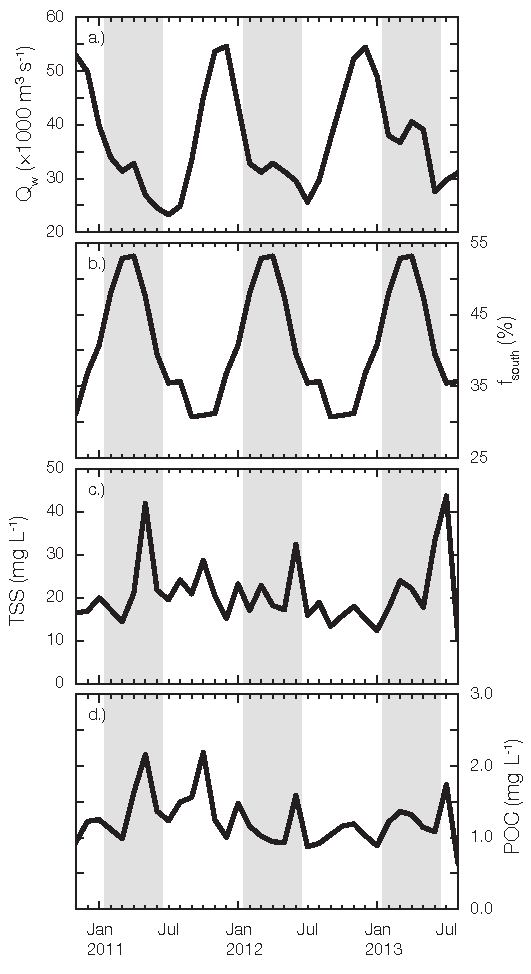
\includegraphics[]{Thesis_Figures/Ch4Fig2}}
	\caption[Environmental parameter time-series plots]{Time series plots of \textit{(A)} Congo River discharge (Q\textsubscript{w}), \textit{(B)} monthly fractional contribution by southern hemisphere tributaries (f\textsubscript{south}) as estimated by \citet{Bricquet:1993ve} (repeating for multiple years), \textit{(C)} TSS concentration, and \textit{(D)} POC concentration measured at Brazzaville/Kinshasa during the sampling period. Southern hemisphere dominated periods are defined when f\textsubscript{south} is greater than the median value of 39\%, and are indicated by gray boxes.}
	\label{Ch4Fig:2} 
\end{figure}

\section{Materials and Methods}

\subsection{Sample collection}

Suspended sediment samples were collected once per month from November 2010 through August 2013 near Brazzaville/Kinshasa, just downstream of Pool Malebo and $\approx 300$ km upstream of the Congo Estuary ($4.3$\textdegree S, $15.3$\textdegree E; Figure \ref{Ch4Fig:1}). The sampling location is downstream of all major tributaries, capturing $>95$\% of the total Congo River catchment, and the effect of the downstream Congo Rapids on bulk organic geochemical properties has been shown to be minimal \citep{Spencer:2012en}. Samples are therefore taken to be representative of material exported to the estuary.

A known volume of surface water ($\approx 25$ L) collected near the center of the channel was filtered through a polyethersulfone (PES) membrane filter (Millipore Corporation) with a nominal pore size of $0.22$ $\mu$m. Filters were dried at $60$\textdegree C for storage and shipment, and sediments were quantitatively re-suspended in $18$M$\Omega$ MilliQ water and freeze-dried in pre-combusted glass jars at $-40$\textdegree C (Christ Alpha-L1 equipped with an in-line cold trap) and weighed for TSS concentration. Discharge was measured concurrently with sample collection via a gauging station operated by the Groupe de Recherche en Sciences Exactes et Naturelles (Republic of Congo) and a rating curve which is periodically updated by Acoustic Doppler Current Profiler (ADCP) transects (Figure \ref{Ch4Fig:2}A). Triplicate transects indicate that precision of discharge measurements is $\pm 5$\%, although overbank flooding during periods of high discharge likely biases measurements towards an underestimate of the true value \citep{Spencer:2014vp}.

\subsection{Extraction, separation, and purification of \textit{n}-alkyl lipids}

After weighing, sediments were homogenized using an agate mortar and pestle and an aliquot was removed for bulk analysis. One sample (June 2013) contained coarse vegetation debris, which was manually removed using solvent-cleaned forceps and weighed separately ($16$ mg; not included in extraction). Sediments were then extracted at $100$\textdegree C for 20 minutes in a microwave accelerated reaction system (MARS, CEM Corporation) in $20$ mL of dichloromethane (DCM) and methanol (9:1). Total lipid extracts were saponified at $70$\textdegree C for 2 hours using $0.5$ M KOH in methanol, after the addition of $\approx$ 1\% $18$M$\Omega$ MilliQ water to prevent methylation of carboxylic acid functional groups. After the addition of $15$ mL of water and $\approx$ 1 g pre-combusted NaCl (to increase density difference), "base" fractions were liquid-liquid extracted in $5$ mL of pure hexane 5 times. Hydrochloric acid was then added until reaching pH $2$, and "acid" fractions were extracted using hexane and DCM (4:1) until the organic phase was clear (generally 5 times). Both acid and base fractions were further purified by column chromatography using $1$ g of Supelclean amino-propyl silica gel (Supelco Analytical) and the following elution scheme: $4$ mL hexane (F1); $7$ mL hexane and DCM (4:1, F2); $10$ mL DCM and acetone (9:1, F3); $14$ mL 2\% (w/w) formic acid in DCM (F4); $18$ mL DCM and methanol (1:1, F5). Acid and base fractions containing alkanes (F1), alcohols (F3), and alkanoic acids (F4) were recombined to ensure maximum recovery.

To isolate \textit{n}-alkanes, F1\textsubscript{T} (acid and base fractions recombined in $1.5$ mL 2:1 hexane:DCM) was subjected to urea adduction in which $500$ $\mu$L of urea-saturated methanol was added and solvent was evaporated using a stream of \ce{N2} gas to promote urea recrystallization (repeated three times). Crystals were rinsed three times with pure hexane to remove the "non adducted" fraction before being dissolved in $15$ mL MilliQ water and liquid-liquid extracted using pure hexane as described above. Both alcohols and alkanoic acids require derivatization in order to be amenable to gas chromatography. Alcohols were acetylated in $250$ $\mu$L of pyridine and acetic anhydride with known isotopic composition (1:1) at $70$\textdegree C for 1 hour. Alkanoic acids were trans-esterified in $15$ mL of HCl and methanol with known isotopic composition (5:95) at $70$\textdegree C for 12 hours. MilliQ water ($15$ mL) was then added, and fatty acid methyl esters (FAMEs) were liquid-liquid extracted into hexane and DCM (4:1) five times. FAMEs were further purified by column chromatography using $1$ g of amino-propyl silica gel eluted with: $4$ mL hexane (F4\textsubscript{T}F1); $7$ mL hexane and DCM (4:1, F4\textsubscript{T}F2); $18$ mL DCM and methanol (1:1, F4\textsubscript{T}F3).

After quantification but before isotope analysis, unsaturated compounds were removed using $0.5$ g silver nitrate silica gel (Supelco Analytical) in a Pasteur pipette column eluted with: $5$ mL hexane and DCM (95:5, SN1); $18$ mL hexane and DCM (4:1, SN2); $5$ mL DCM and acetone (1:1, SN3). Fractions containing \textit{n}-alkanes (F1\textsubscript{T}, adducted), \textit{n}-alcohols (F3\textsubscript{T}, SN2), and \textit{n}-alkanoic acids (F4\textsubscript{T}F2, SN2) were stored at $4$\textdegree C until analyzed. Recovery using this protocol is $\approx 90$\%, as determined by periodically subjecting a known mixture of compounds to the entire procedure.

\subsection{Quantification and isotopic measurements}

Total organic carbon (\%OC) of bulk sediments was measured after decarbonation over HCl fumes at $60$\textdegree C for 72 hours using a Fisons elemental analyzer coupled to a Finnigan Delta\textsuperscript{plus} IRMS as described in \citet{Whiteside:2011jea}. All \textit{n}-alkyl lipids were quantified using a Hewlett Packard 5890 gas chromatograph-flame ionization detector (GC-FID) with a Gerstel PTV injection system, and separated with a VF-1MS capillary column (Agilent Technologies). Temperature program was as follows: ramp to $130$\textdegree C at $30$\textdegree C min\textsuperscript{-1}, ramp to $320$\textdegree C at $8$\textdegree C min\textsuperscript{-1}, hold for 7.5 min at $320$\textdegree C (35min total). Samples were analyzed as a single injection and compared to an external standard run at 3 dilutions between every $\approx$ 5 samples. Uncertainty was calculated using the standard deviation of the best-fit line to the calibration curve.

Compound-specific \ce{\delta^{13}C} was determined using a ThermoFisher Scientific Trace GC Ultra with a DB-1MS capillary column (Agilent Technologies) coupled to a Finnigan MAT252 IRMS via a GC/C combustion interface modified for oxygen trickle flow \citep{Merritt:1995vt,Sessions:2006bn}. Temperature program was as follows: hold for 3 min at $120$\textdegree C, ramp to $200$\textdegree C at $30$\textdegree C min\textsuperscript{-1}, ramp to $320$\textdegree C at $4$\textdegree C min\textsuperscript{-1}, hold for 29.3 min at $320$\textdegree C (70min total). All samples were measured at least in duplicate (triplicate when not limited by low concentrations) and calibrated against pulses of \ce{CO2} gas with a known \ce{\delta^{13}C} value. Long-term precision of an external \textit{n}-alkane standard mixture was $\leq 0.2$\textperthousand\ ($\pm 1\sigma$ standard deviation). Results for individual compounds after correction for derivatization agent are reported with uncertainty as $\pm 1\sigma$ of all injections. Data are reported relative to Vienna Pee-Dee Belemnite (VPDB).

\subsection{Data analysis}

One sample (September 2013) was omitted from the dataset due to contamination by the PES membrane filter, inhibiting the ability to measure bulk \%OC. Additionally, one sample (February 2011) returned spurious \ce{\delta^{13}C} and concentration values, likely due to improper sampling or influence of a local extreme runoff event, and was thus removed in accordance with Chavenet's criterion \citep{Glover:2011tl}. Regressions were performed as weighted least squares (WLS) using a weighting factor of $\sigma^{-1}_{i}$ for each sample $i$ \citep{Glover:2011tl}. All data analysis was performed in the Python programming language v.2.7 and ArcGIS for desktop v.10.3.

\section{Results}

\subsection{Environmental parameters}

All environmental parameters are presented in Table \ref{Ch4Tab:S1}. Congo River discharge recorded at Brazzaville/Kinshasa during the sampling period ranged from a minimum of $23.2 \times 10^3 \pm 1.1 \times 10^3$ m\textsuperscript{3} sec\textsuperscript{-1} in July 2011 to a maximum of $54.6 \times 10^3 \pm 2.7 \times 10^3$ m\textsuperscript{3} sec\textsuperscript{-1} in December 2011 (Figure \ref{Ch4Fig:2}A). Average discharge for 2011 ($35.3 \times 10^3$ m\textsuperscript{3} sec\textsuperscript{-1}) was the fifth-lowest since recording began in 1977, while 2012 and 2013 were closer to long-term average values \citep{Spencer:2012en}. Seasonally, discharge displays two maxima: a large peak in Nov-Dec-Jan during high flow through northern hemisphere tributaries and the main-stem \textit{Cuvette Congolaise}, and a smaller peak in Mar-Apr-May due to increased flow from southern hemisphere tributaries \citep{Bricquet:1993ve,Coynel:2005cn,Bouillon:2012cw,Spencer:2012en,Spencer:2014vp}. This leads to an estimated range in southern-hemisphere contribution (termed f\textsubscript{south}) of 31--53\%, with a median value of 39\% \citep{Bricquet:1993ve}. We classify periods with f\textsubscript{south} above the median value -- \textit{\textit{i.e.}} February through May -- as being "southern hemisphere dominated," and all other times as being "main-stem dominated" or "\textit{Cuvette Congolaise} dominated" (Figure \ref{Ch4Fig:2}B). Importantly, the largest southern-hemisphere tributary, the Kasai River, enters the main-stem downstream of the \textit{Cuvette Congolaise} swamp forest.

TSS concentration averaged $21.1 \pm 7.6$ g m\textsuperscript{-3} throughout the time series, ranging from a minimum of $10.2$ g m\textsuperscript{-3} to a maximum of $43.6$ g m\textsuperscript{-3} (Figure \ref{Ch4Fig:2}C). TSS are rich in carbon, with an average \%OC of $6.1 \pm 1.0$\%, leading to an average particulate organic carbon (POC) concentration of $1.3 \pm 0.4$ g m\textsuperscript{-3} with a range of $0.6 - 2.6$ g m\textsuperscript{-3} (Figure \ref{Ch4Fig:2}D). TSS, POC, and \%OC ranges reported here agree well with published values, both for the main-stem Congo as well as the Oubangui River at Bangui Station (Figure \ref{Ch4Fig:1}), a major right-bank tributary \citep{Coynel:2005cn,Bouillon:2012cw,Bouillon:2014ko}. Congo River suspended sediment \%OC increases slightly as a function of discharge ($R^2 = 0.19$, $p$-value = $0.01$; not shown), although POC concentration shows no correlation with discharge ($p$-value > $0.05$; not shown). 

% Figure 3
\begin{figure}[t]
	\makebox[\textwidth][c]{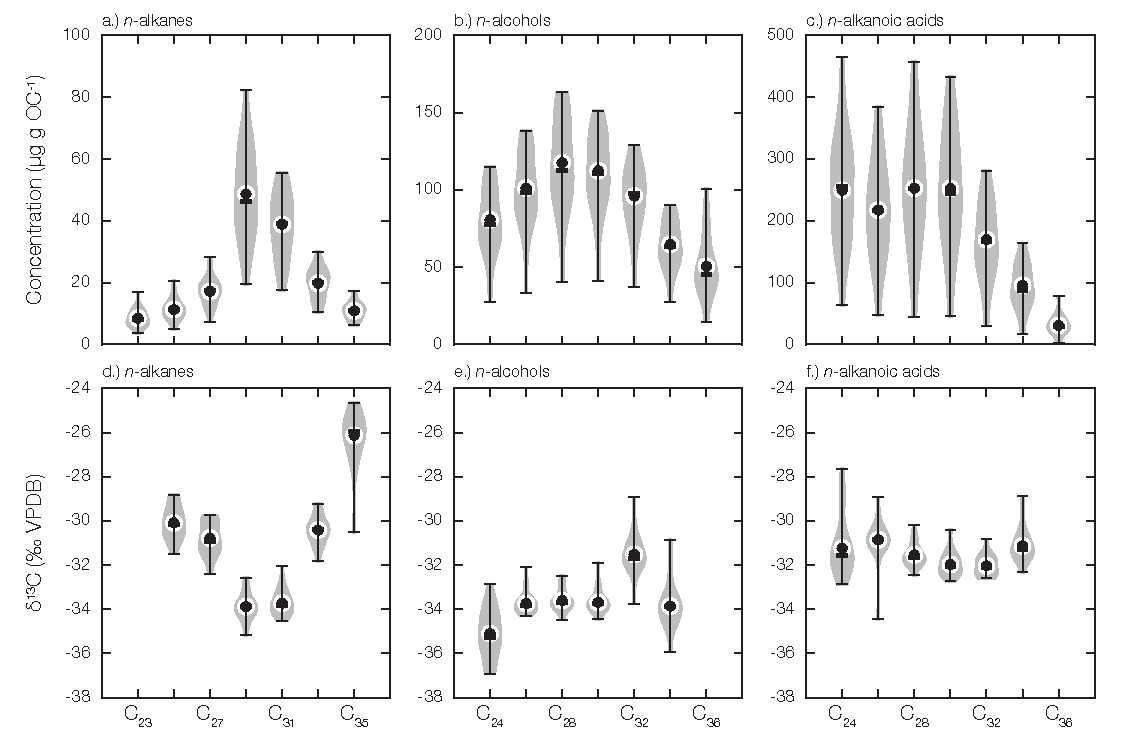
\includegraphics[]{Thesis_Figures/Ch4Fig3}}
	\caption[Concentration and \ce{\delta^{13}C} violin plots]{Violin plots of \textit{n}-alkane, \textit{n}-alcohol, and \textit{n}-alkanoic acid \textit{(A)--(C)} POC-normalized concentrations and \textit{(D)--(F)} \ce{\delta^{13}C} values for individual long-chain homologues. Violin plots represent the temporal distribution of values throughout the time-series using a Gaussian kernel density function. Mean values are marked as black circles, and median values are marked as horizontal black lines.}
	\label{Ch4Fig:3} 
\end{figure}

\subsection{Lipid abundance and distribution}

Concentrations of individual homologues, average chain lengths, and carbon preference indices are presented in Tables \ref{Ch4Tab:S2}--\ref{Ch4Tab:S4}.

\subsubsection{\textit{n}-Alkanes}

Carbon-normalized concentrations of individual plant-wax \textit{n}-alkanes (C\textsubscript{23}--C\textsubscript{35}; odd-numbered homologues) range from a minimum of $3.7 \pm 0.8$ $\mu$g gOC\textsuperscript{-1} (C\textsubscript{23}) to a maximum of $82.1 \pm 1.3$ $\mu$g gOC\textsuperscript{-1} (C\textsubscript{29}; Figure \ref{Ch4Fig:3}A). The sum of the long-chain odd-numbered homologue concentrations ($\Sigma$LC\textsubscript{25-35}) exhibits considerably less variability, ranging from $66.0 - 207.1$ $\mu$g gOC\textsuperscript{-1}. Time-series plots of $\Sigma$LC\textsubscript{25-35} and selected homologue concentrations are presented in Figure \ref{Ch4Fig:4}A--C. $\Sigma$LC\textsubscript{25-35} concentrations show a slight decrease with increasing discharge (Figure \ref{Ch4Fig:5}A), although this relationship is driven by changes in \%OC and disappears when considering sediment-normalized concentrations ($R^2 = 0.001$, $p$-value > $0.05$; not shown).

\textit{n}-Alkanes are consistently dominated by C\textsubscript{29} and C\textsubscript{31} homologues, contributing up to 33\% and 26\% to $\Sigma$LC\textsubscript{25-35}, respectively. At only 8--9\% each, C\textsubscript{25} and C\textsubscript{35} are the least abundant homologues, while C\textsubscript{27} and C\textsubscript{33} contribute 12--13\% each. To compare changes in distributions between samples, we compute the average chain length (ACL) as the concentration-weighted average of C\textsubscript{25}--C\textsubscript{35} odd-numbered homologues:

% Equation 1
\begin{equation}\label{Ch4Eq:1}
\text{ACL} = \frac{25\times[\ce{C}_{25}] + 27\times[\ce{C}_{27}] + 29\times[\ce{C}_{29}] + 31\times[\ce{C}_{31}] + 33\times[\ce{C}_{33}] + 35\times[\ce{C}_{35}]}{\Sigma \text{LC}_{25-35}}
\end{equation}

\textit{n}-Alkane ACL in our sample set is remarkably stable, with an average of $30.0 \pm 0.1$ units and a range of $29.6 - 30.2$ units, and shows no significant correlation with discharge (Figure \ref{Ch4Fig:5}B). We compute the carbon preference index (CPI) for C\textsubscript{25}--C\textsubscript{35}, defined as: 

% Equation 2
\begin{equation}\label{Ch4Eq:2}
\text{CPI} = \frac{1}{2} \left( \frac{\Sigma \text{LC}_{25-35}}{\Sigma \text{LC}_{24-34}} + \frac{\Sigma \text{LC}_{25-35}}{\Sigma \text{LC}_{26-36}} \right)
\end{equation}

$\Sigma$LC\textsubscript{25-35} refers to odd-numbered homologues only while $\Sigma$LC\textsubscript{24-34} and $\Sigma$LC\textsubscript{26-36} refer to even-numbered homologues only (we note that C\textsubscript{36} was not detected in any sample). \textit{n}-Alkane CPI in our dataset averages $2.9 \pm 0.5$, ranging from $2.1 - 4.1$, and shows a small yet statistically significant decrease with increasing discharge (Figure \ref{Ch4Fig:5}C).

We additionally calculate P\textsubscript{aq}, an estimate of macrophyte contribution to \textit{n}-alkanes \citep{Ficken:2000wq} as:

% Equation 3
\begin{equation}\label{Ch4Eq:3}
\text{P}_{\text{aq}} = \frac{[\ce{C}_{23}] + [\ce{C}_{25}]}{[\ce{C}_{23}] + [\ce{C}_{25}] + [\ce{C}_{27}] + [\ce{C}_{29}]}
\end{equation}

Resulting P\textsubscript{aq} values in our sample set (Table \ref{Ch4Tab:S2}) average $0.19 \pm 0.04$ with a range of $0.12 - 0.26$, and are uncorrelated with discharge ($R^2 = 0.08$, $p$-value > $0.05$; not shown).

% Figure 4
\begin{figure}[p]
	\makebox[\textwidth][c]{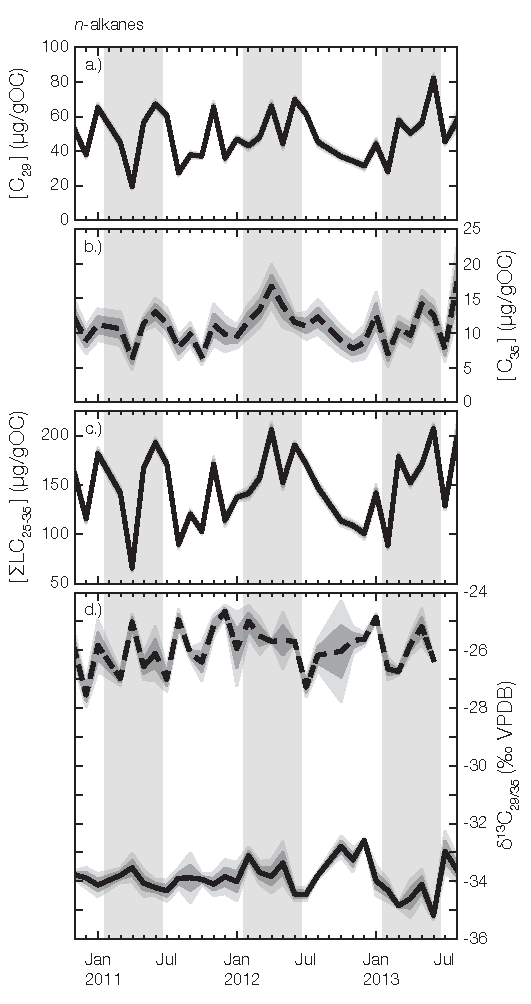
\includegraphics[]{Thesis_Figures/Ch4Fig4}}
	\caption[\textit{n}-alkane concentration and \ce{\delta^{13}C} time-series plots]{Time series plots of \textit{n}-alkane concentrations -- \textit{(A)} C\textsubscript{29}, \textit{(B)} C\textsubscript{35}, \textit{(C)} $\Sigma$LC\textsubscript{25-35} -- and \ce{\delta^{13}C} values -- \textit{(D)} C\textsubscript{29} (solid line) and C\textsubscript{35} (dashed line). Selected homologues are chosen to represent the increasing influence by C\textsubscript{4} grasses with increasing chain length. Dark gray shading represents $\pm 1\sigma$ uncertainty, and light gray shading represents 95\% confidence interval (CI). Periods when f\textsubscript{south} > 39\% are indicated by gray boxes.}
	\label{Ch4Fig:4} 
\end{figure}

% Figure 5
\begin{figure}[p]
	\makebox[\textwidth][c]{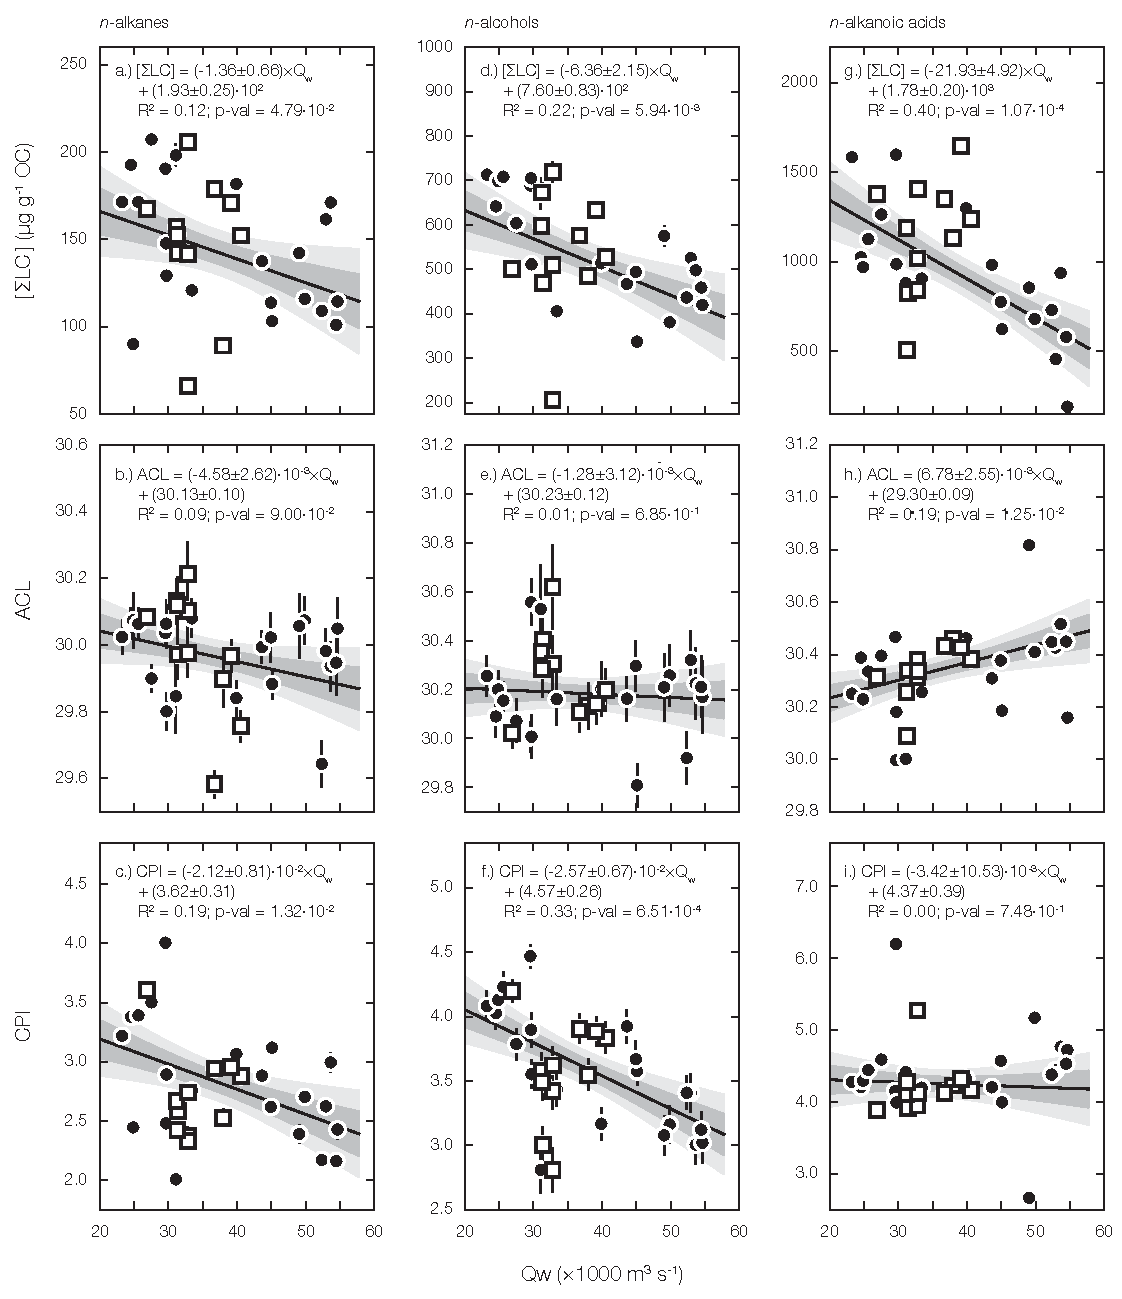
\includegraphics[scale=0.9]{Thesis_Figures/Ch4Fig5}}
	\caption[Correlations between concentration, ACL, CPI, and discharge]{Correlations between $\Sigma$LC\textsubscript{25-35}/$\Sigma$LC\textsubscript{26-36} concentrations, ACL, and CPI vs. Congo River discharge (Q\textsubscript{w}) measured at Brazzaville/Kinshasa for \textit{n}-alkanes \textit{(A)--(C)}, \textit{n}-alcohols \textit{(D)--(F)}, and \textit{n}-alkanoic acids \textit{(G)--(I)}. Error bars on individual points represent $\pm 1 \sigma$ uncertainty. Black line is the WLS best-fit line, dark gray shading represents $\pm 1 \sigma$  regression uncertainty, and light gray shading represents the 95\% CI. Samples collected when f\textsubscript{south} > 39\% are plotted as white squares, and samples collected when f\textsubscript{south} $\leq$ 39\% are plotted as black circles.}
	\label{Ch4Fig:5} 
\end{figure}

\subsubsection{\textit{n}-Alcohols}

While nominally regarded as a plant-wax lipid, C\textsubscript{24} \textit{n}-alcohol has been observed in freshwater phytoplankton \citep{Volkman:1998tk,Volkman:1999tq,Xu:2007jk}. In our sample set, isotopic evidence indicates that phytoplankton contribute to C\textsubscript{24} \textit{n}-alcohol (see section \ref{Ch4Sec:52} below), and we therefore omit this compound from our calculations of ACL, CPI, and $\Sigma$LC. 

Plant-wax \textit{n}-alcohols (C\textsubscript{26}--C\textsubscript{36}; even-numbered homologues) are considerably more abundant than \textit{n}-alkanes, with individual compound concentrations ranging from $14.6 \pm 3.1$ $\mu$g gOC\textsuperscript{-1} (C\textsubscript{36}) to $163.0 \pm 8.0$ $\mu$g gOC\textsuperscript{-1} (C\textsubscript{28}; Figure \ref{Ch4Fig:3}B). $\Sigma$LC\textsubscript{26-36} concentrations range from $206.5 - 718.7$ $\mu$g gOC\textsuperscript{-1}, and are therefore $3.8 \pm 0.9$ times higher than corresponding \textit{n}-alkane concentrations. Time series plots of $\Sigma$LC\textsubscript{26-36} and selected homologue concentrations are shown in Figure \ref{Ch4Fig:6}A--C, while Figure \ref{Ch4Fig:5}D shows that $\Sigma$LC\textsubscript{26-36} concentrations decrease as a function of river discharge. Again, this relationship is driven by changes in \%OC, as sediment-normalized $\Sigma$LC\textsubscript{26-36} concentrations display no significant relationship with discharge ($R^2 = 0.04$, $p$-value > $0.05$; not shown).

\textit{n}-Alcohols are more evenly distributed than \textit{n}-alkanes, with no single homologue contributing more than 21\% or less than 9\% of the long-chain total (Figure \ref{Ch4Fig:3}B). ACL is calculated similarly to \textit{n}-alkanes, but using C\textsubscript{26}--C\textsubscript{36} even-numbered homologues. Again, ACL shows little variability, with a range of $29.8 - 30.6$ units and an average of $30.2 \pm 0.2$ units. CPI, calculated as above but using $\Sigma$LC\textsubscript{26-36} in the numerator and $\Sigma$LC\textsubscript{25-35}/$\Sigma$LC\textsubscript{27-37} in the denominators (noting that C\textsubscript{37} was not detected in any sample), averages $3.7 \pm 0.4$ with a range of $3.0 - 4.6$. While ACL shows no correlation (Figure \ref{Ch4Fig:5}E), CPI exhibits a strong negative relationship with discharge (Figure \ref{Ch4Fig:5}F).

% Figure 6
\begin{figure}[p]
	\makebox[\textwidth][c]{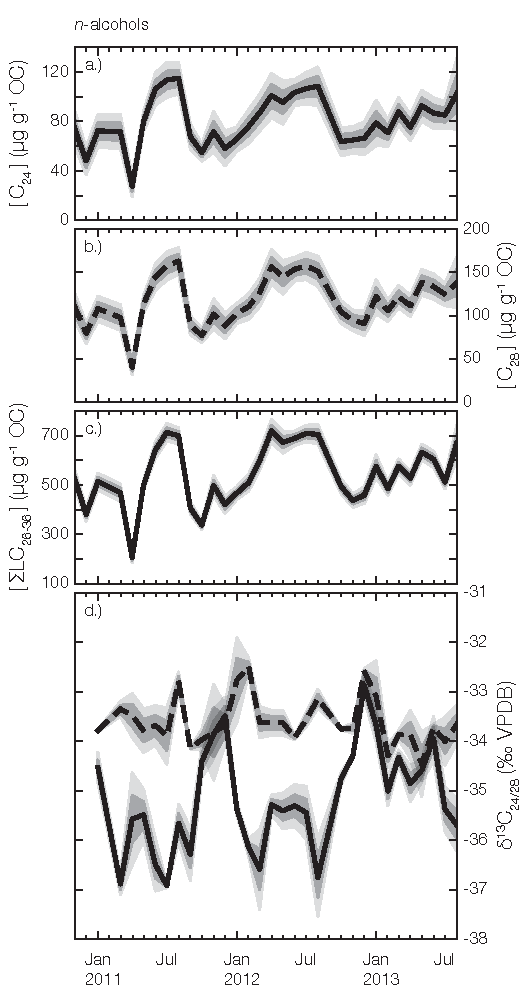
\includegraphics[]{Thesis_Figures/Ch4Fig6}}
	\caption[\textit{n}-alcohol concentration and \ce{\delta^{13}C} time-series plots]{Time series plots of \textit{n}-alcohol concentrations -- \textit{(A)} C\textsubscript{24}, \textit{(B)} C\textsubscript{28}, \textit{(C)} $\Sigma$LC\textsubscript{26-36} -- and \ce{\delta^{13}C} values -- \textit{(D)} C\textsubscript{24} (solid line) and C\textsubscript{28} (dashed line). Selected homologues are chosen to represent the autochthonous contribution to C\textsubscript{24} and C\textsubscript{3} plant dominance of longer homologues. Dark gray shading represents $\pm 1\sigma$ uncertainty, and light gray shading represents 95\% confidence interval (CI). Periods when f\textsubscript{south} > 39\% are indicated by gray boxes.}
	\label{Ch4Fig:6} 
\end{figure}

\subsubsection{\textit{n}-Alkanoic acids}

As C\textsubscript{24} \textit{n}-alcohol was omitted from the above calculations, to accurately compare ACL, CPI, and $\Sigma$LC across compound classes we remove C\textsubscript{24} \textit{n}-alkanoic acid from the calculations performed here.

Plant-wax \textit{n}-alkanoic acid concentrations (C\textsubscript{26}--C\textsubscript{36}; even-numbered homologues) display the highest values and largest variability of all \textit{n}-alkyl lipid classes (Figure \ref{Ch4Fig:3}C). Individual compounds range from $2.7 \pm 0.2$ $\mu$g gOC\textsuperscript{-1} (C\textsubscript{36}) to $457.1 \pm 2.3$ $\mu$g gOC\textsuperscript{-1} (C\textsubscript{28}), with a $\Sigma$LC\textsubscript{26-36} concentration range of $190.2 - 1648.6$ $\mu$g gOC\textsuperscript{-1}. Long-chain \textit{n}-alkanoic acids therefore contribute up to $\approx 0.2$\% of total exported POC, and are $7.1 \pm 2.5$ times more abundant than \textit{n}-alkanes. Similar to \textit{n}-alkanes and \textit{n}-alcohols, \textit{n}-alkanoic acid carbon-normalized $\Sigma$LC\textsubscript{26-36} concentrations decrease with increasing river discharge (Figure \ref{Ch4Fig:5}G). While this relationship is partially driven by changes in \%OC, sediment-normalized values additionally exhibit a statistically significant decrease ($R^2 = 0.19$, $p$-value = $1.4 \times 10^{-2}$; not shown). Time series plots of selected homologues and $\Sigma$LC\textsubscript{26-36} concentrations are plotted in Figure \ref{Ch4Fig:7}A--C.

\textit{n}-Alkanoic acids display a similar distribution to \textit{n}-alcohols, with C\textsubscript{26}, C\textsubscript{28}, and C\textsubscript{30} all contributing $\approx 20 - 25$\% of the long-chain total, and decreasing contribution with increasing chain length beyond C\textsubscript{30} (Figure \ref{Ch4Fig:3}C). Average ACL is $29.5 \pm 0.2$, slightly lower than that of \textit{n}-alkanes and \textit{n}-alcohols, and exhibits a slight increase with increasing discharge (Figure \ref{Ch4Fig:5}H). \textit{n}-Alkanoic acid CPI is the highest of all observed compound classes (C\textsubscript{37} not detected), averaging $4.3 \pm 0.5$ and shows no correlation with river discharge (Figure \ref{Ch4Fig:5}I). We note that inclusion of \textit{n}-C\textsubscript{24} decreases ACL to $28.4 \pm 0.2$ and exhibits no effect on CPI (not shown).

% Figure 7
\begin{figure}[p]
	\makebox[\textwidth][c]{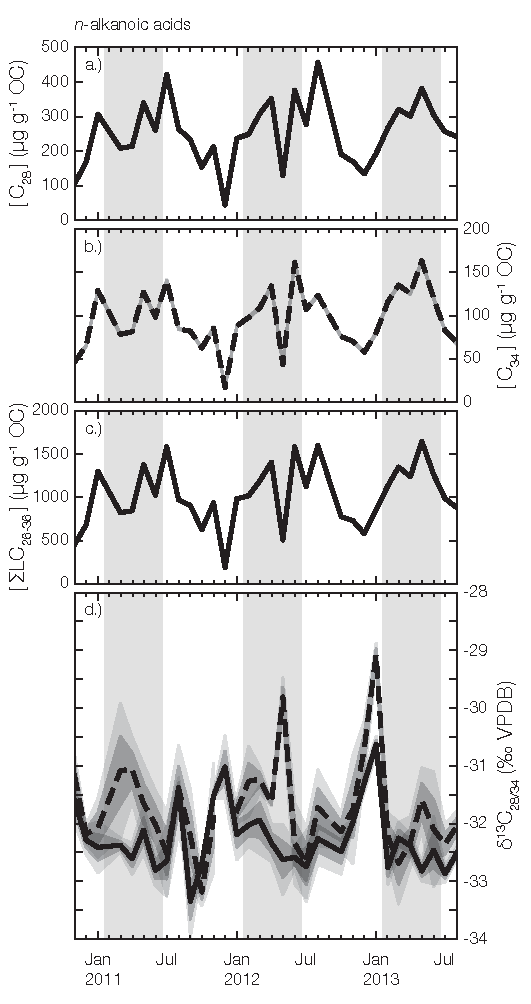
\includegraphics[]{Thesis_Figures/Ch4Fig7}}
	\caption[\textit{n}-alkanoic acid concentration and \ce{\delta^{13}C} time-series plots]{Time series plots of \textit{n}-alkanoic acid concentrations -- \textit{(A)} C\textsubscript{28}, \textit{(B)} C\textsubscript{34}, \textit{(C)} $\Sigma$LC\textsubscript{26-36} -- and \ce{\delta^{13}C} values -- \textit{(D)} C\textsubscript{28} (solid line) and C\textsubscript{34} (dashed line). Selected homologues are chosen to represent the similar C\textsubscript{3}-like isotopic composition across all long-chain homologues. Dark gray shading represents $\pm 1\sigma$ uncertainty, and light gray shading represents 95\% confidence interval (CI). Periods when f\textsubscript{south} > 39\% are indicated by gray boxes.}
	\label{Ch4Fig:7}
\end{figure}

\subsection{Compound-specific \ce{\delta^{13}C}}

Individual homologue \ce{\delta^{13}C} measurements are reported in Tables \ref{Ch4Tab:S5}--\ref{Ch4Tab:S7}.

\subsubsection{\textit{n}-Alkanes}

\textit{n}-Alkanes display the largest \ce{\delta^{13}C} variability across long-chain homologues of all compound classes studied, with an average spread (max -- min) of $8.1 \pm 0.7$\textperthousand\ (Figure \ref{Ch4Fig:3}D). However, we note that C\textsubscript{25} could not be measured in two samples (December 2010, July 2013) and C\textsubscript{35} could not be measured in one sample (July 2013), as concentrations were too low. All samples show the same general trend with chain length -- \textit{i.e.} C\textsubscript{25}, C\textsubscript{27}, and C\textsubscript{33} near $-30$\textperthousand, C\textsubscript{29} and C\textsubscript{31} near $-34$\textperthousand, and C\textsubscript{35} up to $-24.7 \pm 0.1$\textperthousand\ (Figure \ref{Ch4Fig:3}D). Temporal variability for each compound in the dataset is $\approx 2.5 - 3.0$\textperthousand\ (max -- min), as is shown for C\textsubscript{29} and C\textsubscript{35} in Figure \ref{Ch4Fig:4}D. \ce{\delta^{13}C} values of all compounds are uncorrelated with discharge ($p$-value > $0.05$; not shown).

\subsubsection{\textit{n}-Alcohols}

Low concentrations prevented the measurement of \ce{\delta^{13}C} values for C\textsubscript{36} \textit{n}-alcohol. Additionally, one sample (December 2010) displayed contamination by siloxanes and was omitted. All remaining samples follow the same general pattern, with C\textsubscript{24} exhibiting the most depleted values, nearly identical values for C\textsubscript{26}--C\textsubscript{30} and C\textsubscript{34}, and C\textsubscript{32} showing the most enrichment, averaging $-31.1 \pm 0.7$\textperthousand\ (Figure \ref{Ch4Fig:3}E).

Time series plots of \ce{\delta^{13}C} values for C\textsubscript{24} and C\textsubscript{28} \textit{n}-alcohols are plotted in Figure \ref{Ch4Fig:6}D. C\textsubscript{24} \ce{\delta^{13}C} values display a strong positive correlation with discharge (Figure \ref{Ch4Fig:8}A), with the most \ce{^{13}C}-depleted value ($-36.9 \pm 0.1$\textperthousand) observed during the lowest measured discharge on record (July 2011). In contrast, C\textsubscript{28}--C\textsubscript{34} \ce{\delta^{13}C} values display no correlation with discharge ($p$-value > $0.05$; not shown), although C\textsubscript{26} exhibits a slight positive relationship, mainly driven by three outlier points (Figure \ref{Ch4Fig:8}B). Resulting \ce{\delta^{13}C} spread across measured plant-wax \textit{n}-alcohols (\textit{\textit{i.e.}} C\textsubscript{26}--C\textsubscript{34}) is therefore $2.6 \pm 0.6$\textperthousand, significantly lower than that for \textit{n}-alkanes, even when only considering analogous homologues (\textit{i.e.} C\textsubscript{25}--C\textsubscript{33} \textit{n}-alkane spread of $4.2 \pm 0.6$\textperthousand). While temporal variability within C\textsubscript{26}--C\textsubscript{30} homologues is $\approx 2.5$\textperthousand, C\textsubscript{32} and C\textsubscript{34} are significantly more variable, with a max -- min value of $\approx 3.5$\textperthousand. 

% Figure 8
\begin{figure}[p]
	\makebox[\textwidth][c]{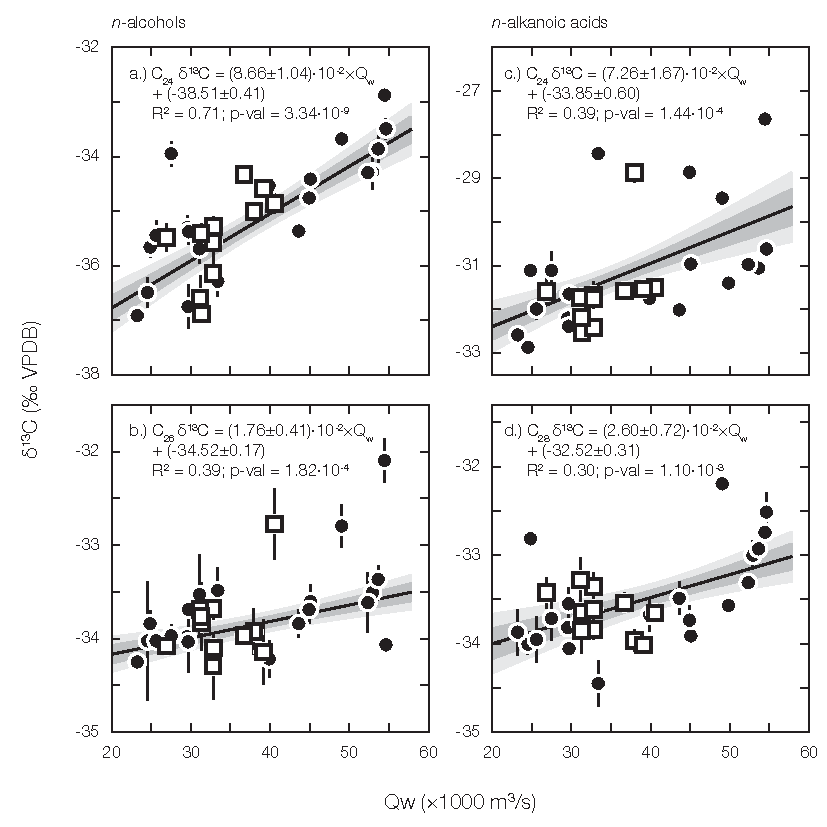
\includegraphics[]{Thesis_Figures/Ch4Fig8}}
	\caption[Correlations between \ce{\delta^{13}C} and discharge]{Correlations between \ce{\delta^{13}C} values vs. Congo River discharge (Q\textsubscript{w}) measured at Brazzaville/Kinshasa for \textit{(A)} C\textsubscript{24} \textit{n}-alcohol, \textit{(B)} C\textsubscript{26} \textit{n}-alcohol, \textit{(C)} C\textsubscript{24} \textit{n}-alkanoic acid, and \textit{(D)} C\textsubscript{28} \textit{n}-alkanoic acid. Error bars on individual points represent $\pm 1 \sigma$ uncertainty. Black line is the WLS best-fit line, dark gray shading represents $\pm 1 \sigma$ regression uncertainty, and light gray shading represents the 95\% CI. Samples collected when f\textsubscript{south} > 39\% are plotted as white squares, and samples collected when f\textsubscript{south} $\leq$ 39\% are plotted as black circles.}
	\label{Ch4Fig:8} 
\end{figure}

\subsubsection{\textit{n}-Alkanoic acids}

C\textsubscript{36} \textit{n}-alkanoic acid \ce{\delta^{13}C} values could not be measured as concentrations were too low, nor could C\textsubscript{34} in one sample (December 2011). Similar to \textit{n}-alcohols, \textit{n}-alkanoic acids show significantly less spread in \ce{\delta^{13}C} values between measured homologues (\textit{i.e.} C\textsubscript{24}--C\textsubscript{34}; $2.0 \pm 1.1$\textperthousand) than do \textit{n}-alkanes (Figure \ref{Ch4Fig:3}F). C\textsubscript{24} and C\textsubscript{26} \textit{n}-alkanoic acids display the largest temporal variability of all measured compounds with a range of $5.2$\textperthousand\ and $5.5$\textperthousand, respectively. In contrast, C\textsubscript{28}--C\textsubscript{32} temporal variability is $\approx 2.5$\textperthousand, similar to that for \textit{n}-alkanes and \textit{n}-alcohols, while C\textsubscript{34} varies by $3.4$\textperthousand\ (Figure \ref{Ch4Fig:7}D).

Unlike \textit{n}-alcohols, C\textsubscript{24} \textit{n}-alkanoic acids do not show \ce{^{13}C}-depletion relative to longer chain homologues during periods of low discharge ($p$-value > $0.05$; not shown). In addition, C\textsubscript{24}--C\textsubscript{26} \textit{n}-alkanoic acids are \ce{^{13}C}-eriched relative to C\textsubscript{24} \textit{n}-alcohol by $3.9 \pm 1.1$\textperthousand\ and $4.3 \pm 1.3$\textperthousand, respectively. C\textsubscript{24} and C\textsubscript{28} \ce{\delta^{13}C} values show a small yet statistically significant enrichment with increasing discharge (Figure \ref{Ch4Fig:8}C--D), while all other compounds are uncorrelated ($p$-value > $0.05$; not shown).

\subsection{Correlations between homologues and compound classes}

WLS regression correlation coefficients ($r$) and significance $p$-values for concentrations and \ce{\delta^{13}C} values of each compound are presented in Tables \ref{Ch4Tab:1}--\ref{Ch4Tab:3}. 

Within each \textit{n}-alkyl compound class, concentrations of all long-chain homologues exhibit statistically significant positive correlations, with $r$ ranging from $0.52 - 0.94$ for \textit{n}-alkanes, $0.71 - 0.98$ for \textit{n}-alcohols, and $0.70 - 0.99$ for \textit{n}-alkanoic acids. In contrast, concentrations of long-chain homologues between different compound classes are uncorrelated or display weak positive correlation ($r \leq 0.75$). Concentrations of both C\textsubscript{23} and C\textsubscript{25} \textit{n}-alkane are statistically uncorrelated with their corresponding (\textit{i.e.} $n + 1$) \textit{n}-alkanoic acids. Additionally, C\textsubscript{23}, C\textsubscript{25}, and C\textsubscript{35} \textit{n}-alkane concentrations are uncorrelated with those of C\textsubscript{28}--C\textsubscript{34} \textit{n}-alkanoic acid; C\textsubscript{36} \textit{n}-alcohol is uncorrelated with C\textsubscript{30}--C\textsubscript{36} \textit{n}-alkanoic acid; and C\textsubscript{29} \textit{n}-alkane is uncorrelated with C\textsubscript{36} \textit{n}-alcohol, indicating a decoupling between the sources of these compounds.

In general, \ce{\delta^{13}C} values between all long-chain homologues exhibit less correlation than do concentrations. Within each compound class, $r$ exhibits a range of $-0.02$ to $0.75$ for \textit{n}-alkanes, $-0.09$ to $0.50$ for \textit{n}-alcohols, and $-0.55$ to $0.79$ for \textit{n}-alkanoic acids. Similar ranges are observed between compound classes: $-0.09$ to $0.78$ between \textit{n}-alkanes and \textit{n}-alcohols, $-0.16$ to $0.63$ between \textit{n}-alkanes and \textit{n}-alkanoic acids, and $-0.35$ to $0.58$ between \textit{n}-alcohols and \textit{n}-alkanoic acids. Interestingly, \ce{\delta^{13}C} values between C\textsubscript{26} and C\textsubscript{34} \textit{n}-alkanoic acids display a statistically significant negative correlation, while all other significant correlations are positive.

Lastly, \ce{\delta^{13}C} values are generally either uncorrelated with concentrations or display a statistically significant negative correlation. C\textsubscript{27}--C\textsubscript{33} \textit{n}-alkane, C\textsubscript{24} \textit{n}-alcohol, and C\textsubscript{24} \textit{n}-alkanoic acid \ce{\delta^{13}C} values all exhibit significant negative correlation with increasing concentrations of most measured compounds, while C\textsubscript{25} \textit{n}-alkane, C\textsubscript{35} \textit{n}-alkane, C\textsubscript{28}--C\textsubscript{30} \textit{n}-alcohol, and C\textsubscript{34} \textit{n}-alcohol \ce{\delta^{13}C} values are statistically uncorrelated with the concentrations of all compounds. In contrast to other compound classes, some \textit{n}-alkanoic acid \ce{\delta^{13}C} values exhibit significant positive correlation with concentrations: C\textsubscript{30} \ce{\delta^{13}C} values correlate positively with C\textsubscript{33}--C\textsubscript{35} \textit{n}-alkane and C\textsubscript{36} \textit{n}-alcohol concentrations, C\textsubscript{32} \ce{\delta^{13}C} values correlate positively with C\textsubscript{36} \textit{n}-alcohol concentrations, and C\textsubscript{34} \ce{\delta^{13}C} values correlate positively with C\textsubscript{36} \textit{n}-alkanoic acid concentrations. 

% Table 1
\begin{sidewaystable}[p]
	\caption[C\textsubscript{23+} concentration correlation $r$ and $p$-values]{Weighted least squares regression correlation values ($r$) and significance $p$-values between all measured C\textsubscript{23+} \textit{n}-alkyl lipid concentrations. Statistically significant ($p$-value $\leq  0.05$) correlations are bolded.}
	\centering
		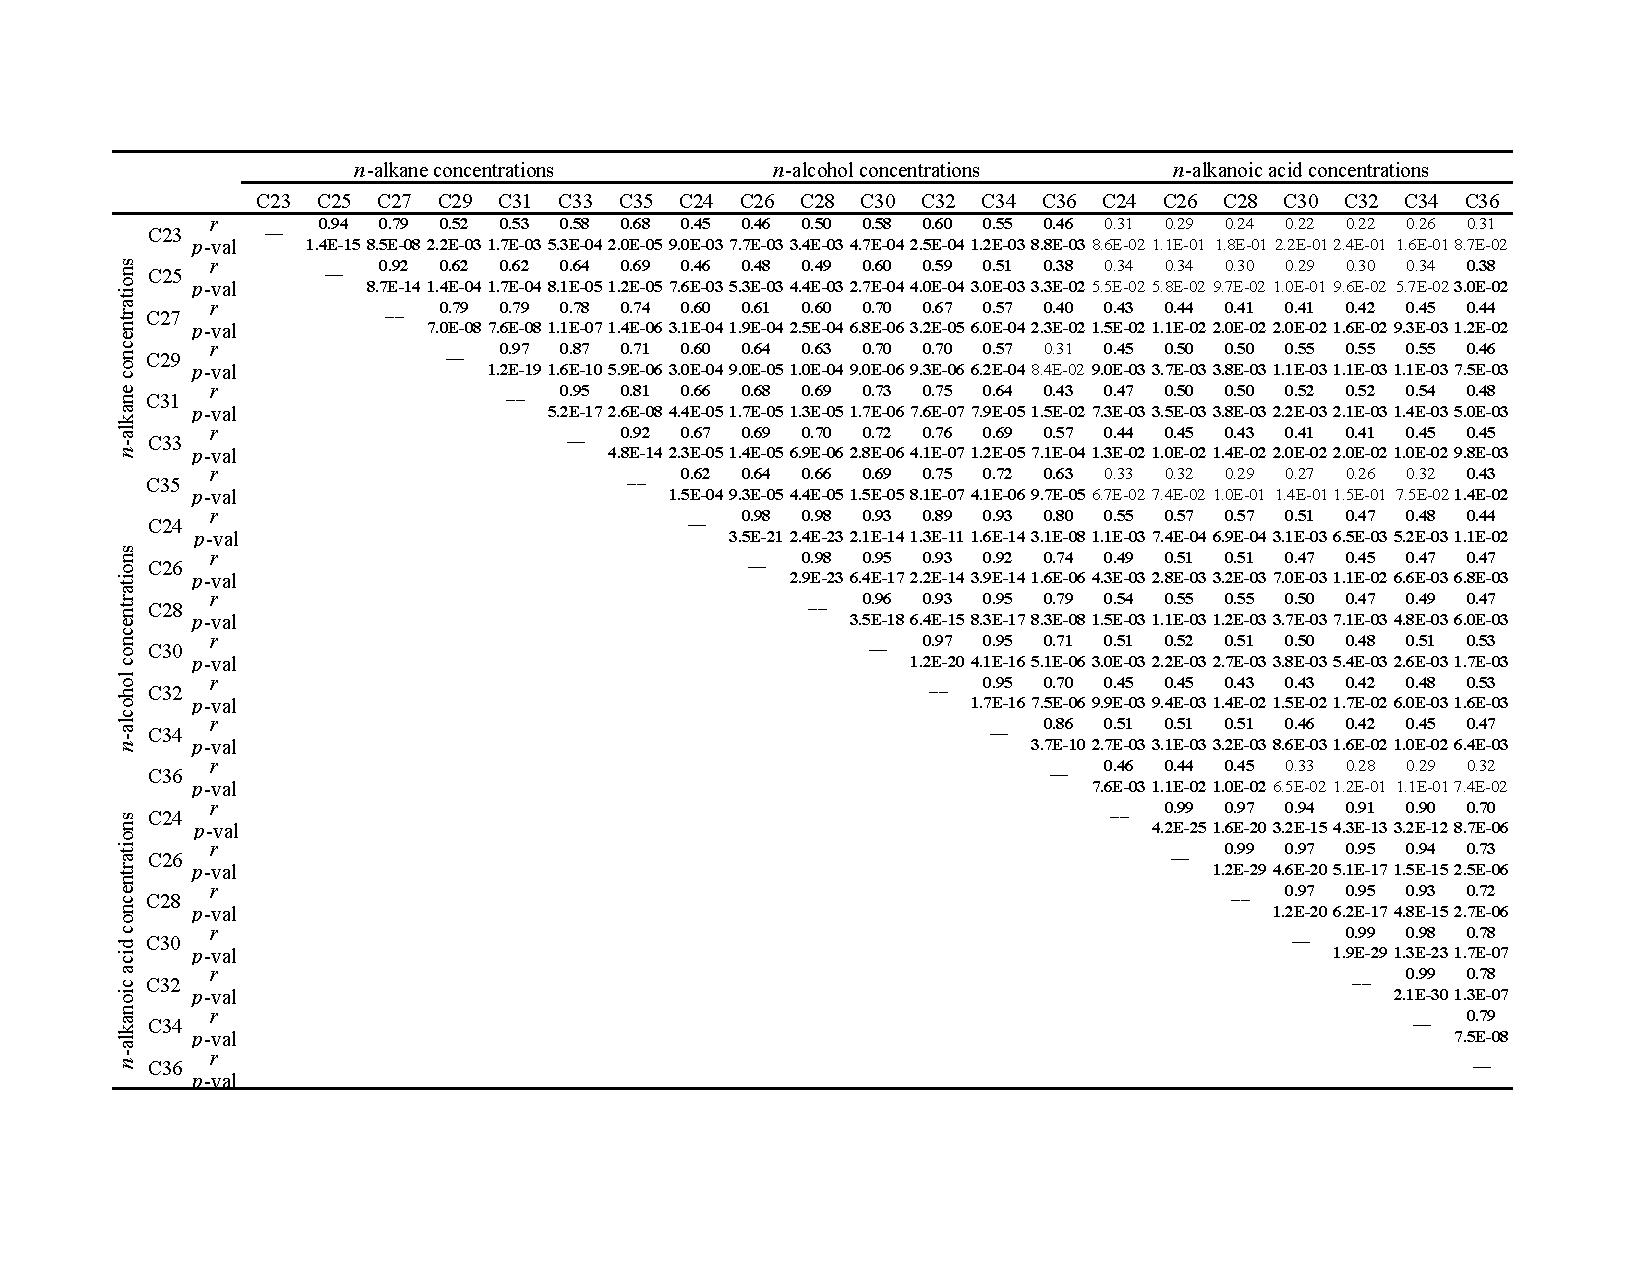
\includegraphics{Thesis_Tables/Ch4Tab1}
	\label{Ch4Tab:1} 
\end{sidewaystable}

% Table 2
\begin{sidewaystable}[p]
	\caption[C\textsubscript{25+} \ce{\delta^{13}C} correlation $r$ and $p$-values]{Weighted least squares regression correlation values ($r$) and significance $p$-values between all measured C\textsubscript{25+} \textit{n}-alkyl lipid \ce{\delta^{13}C} values. Statistically significant ($p$-value $\leq  0.05$) correlations are bolded.}
	\centering
		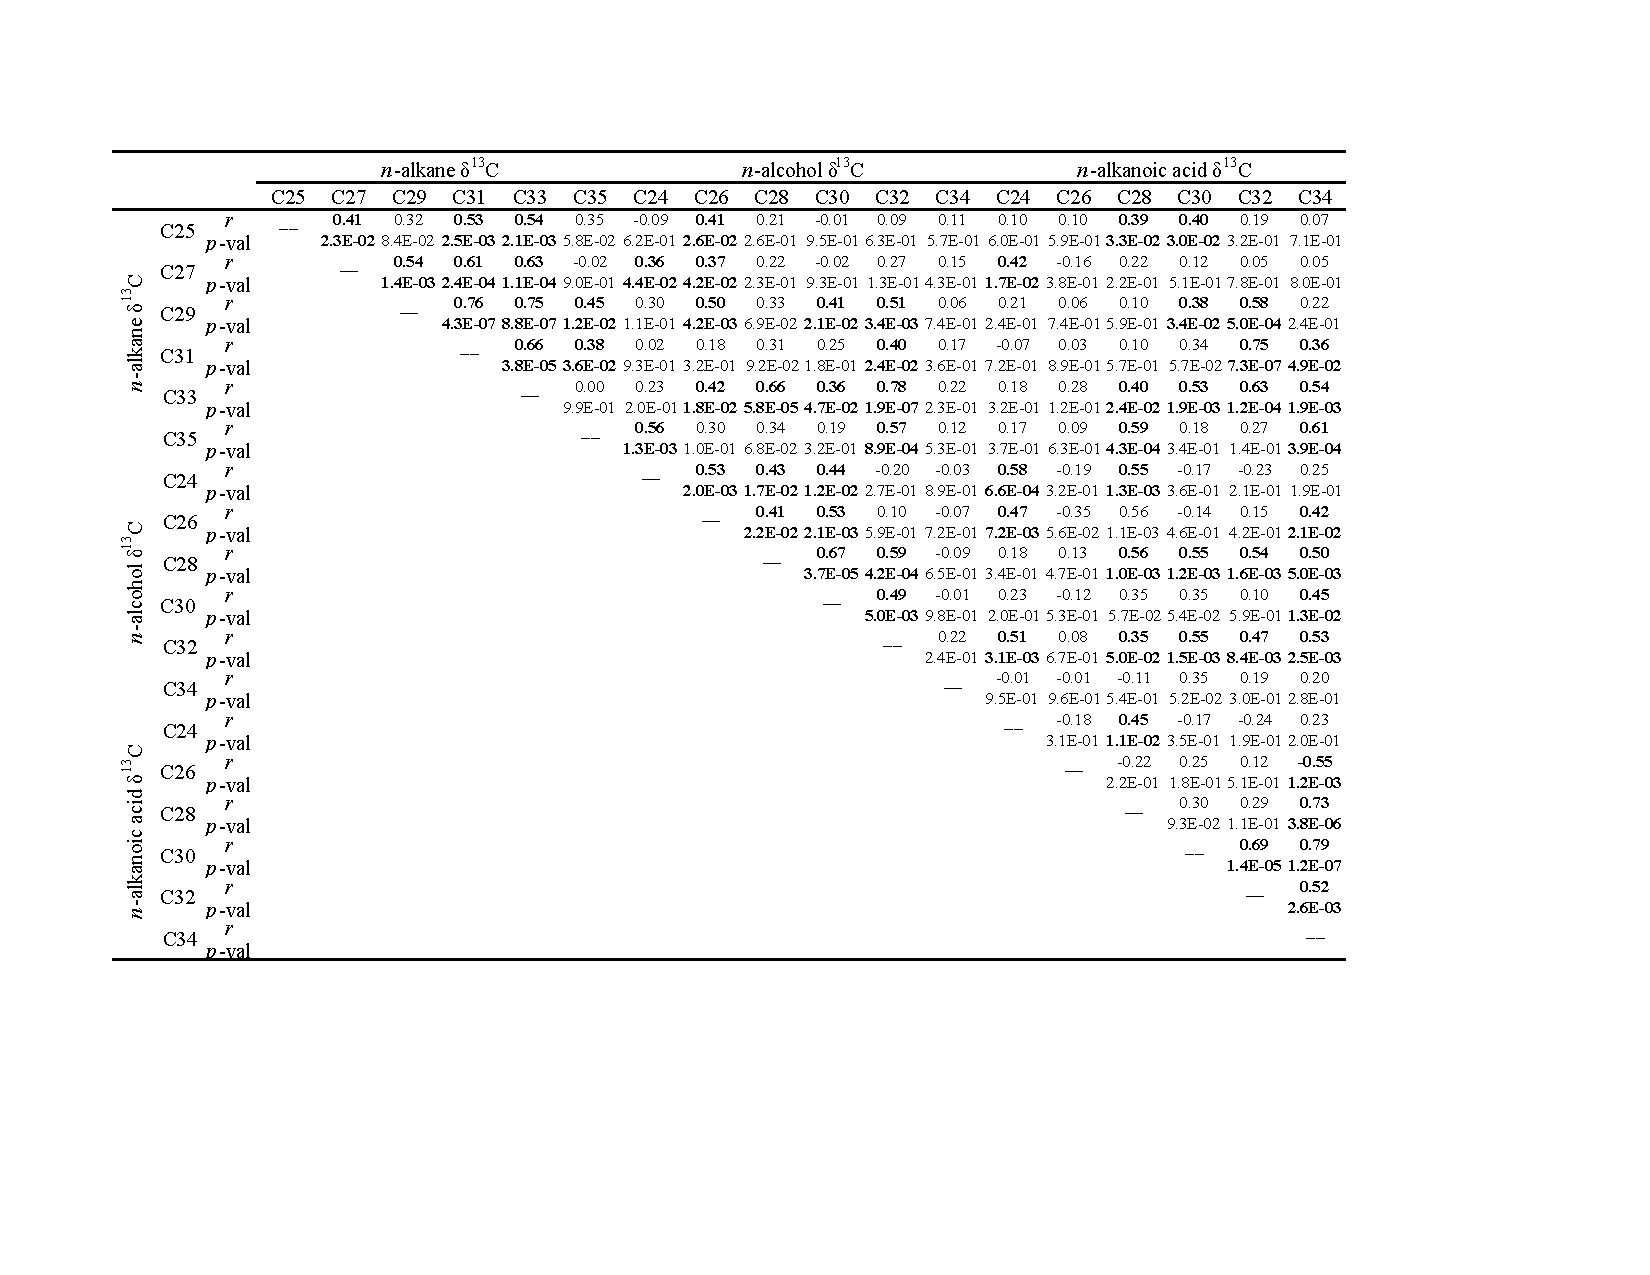
\includegraphics{Thesis_Tables/Ch4Tab2}
	\label{Ch4Tab:2} 
\end{sidewaystable}

% Table 3
\begin{sidewaystable}[p]
	\caption[C\textsubscript{25+} concentration vs. \ce{\delta^{13}C} correlation $r$ and $p$-values]{Weighted least squares regression correlation values ($r$) and significance $p$-values between all measured C\textsubscript{23+} \textit{n}-alkyl lipid concentrations vs. C\textsubscript{25+} \ce{\delta^{13}C} values. Statistically significant ($p$-value $\leq  0.05$) correlations are bolded.}
	\centering
		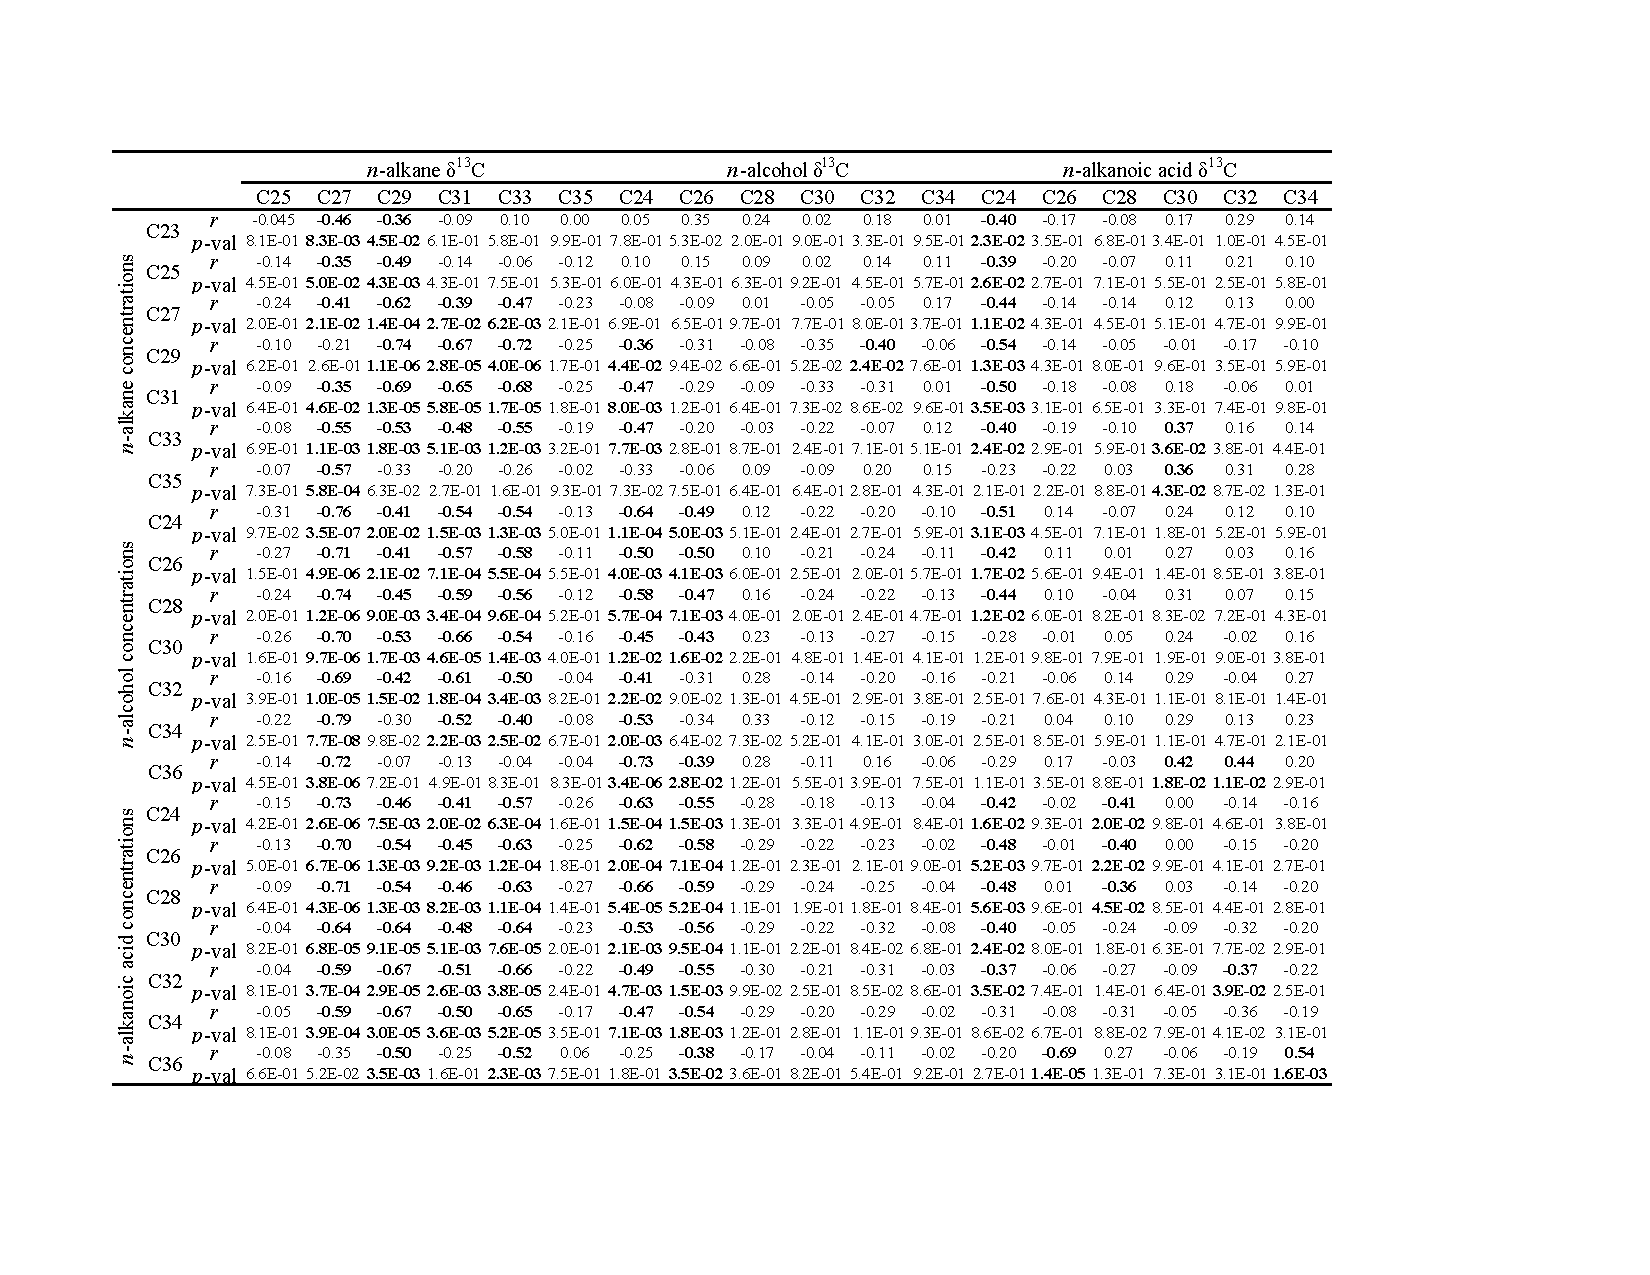
\includegraphics{Thesis_Tables/Ch4Tab3}
	\label{Ch4Tab:3} 
\end{sidewaystable}

\section{Discussion}

\subsection{\textit{n}-Alkane homologues variably record a spatially integrated signal}

Contrary to \textit{n}-alcohols and \textit{n}-alkanoic acids, Congo River carbon-normalized \textit{n}-alkane concentrations are relatively low compared to other large rivers studied \citep{vanDongen:2008kj,Galy:2011ix,Tao:2015bq}. In addition to vascular plants, petrogenic sources can also contribute to alkanes, especially even chain-length saturated homologues due to the low CPI value ($\approx 1.0$) of rock-derived sources as compared to plant waxes \citep{Eglinton:1967uz,Brooks:1969wh}. Low concentrations prevented the measurement of even chain-length \ce{\delta^{13}C} values in our samples, however CPI values between $2.1$ and $4.1$ indicate that \textit{n}-alkanes are dominated by a vascular plant signal. Additionally, the Congo catchment is composed mainly of Neoproterozoic craton lithology and exhibits low catchment relief, precluding a significant contribution of outcropped sedimentary rocks to Congo River suspended sediments \citep{Milliman:2011ug,Galy:2015fx}. Due to their lack of functional groups, \textit{n}-alkanes are more resistant to diagenetic degradation within soils and sediments than are \textit{n}-alkanoic acids and \textit{n}-alcohols \citep{Cranwell:1981vg,Meyers:1993up,Meyers:1993vwa, SinningheDamste:2002ud,vanDongen:2008kj}. For example, \citet{Hoefs:2002wu} show that \textit{n}-alkanes exhibit $\approx 3\times$ higher preservation factors than do \textit{n}-alkanoic acids upon re-exposure of anoxic sediments to oxygen, while \citet{Canuel:1996ta} and \citet{Sun:1994wj} calculate lower degradation rates for \textit{n}-alkanes than for functionalized lipids in both oxic and anoxic surface sediments. These results are consistent with observed pre-aging of \textit{n}-alkanes prior to fluvial export, as indicated by $^{14}$C-derived ages of plant-wax \textit{n}-alkanes in suspended sediments from other large rivers \citep[\textit{e.g.}][]{Gustafsson:2011ht,Tao:2015bq}.

Congo River suspended sediment \textit{n}-alkanes exhibit significantly lower CPI values than do \textit{n}-alcohols and \textit{n}-alkanoic acids (Figure \ref{Ch4Fig:5}C, \ref{Ch4Fig:5}F, \ref{Ch4Fig:5}I), suggesting increased exposure to diagenesis \citep{Meyers:1993vwa}. Additionally, a compilation of individual African forb, grass, shrub, and tree leaves indicates significant overlap in long-chain (\textit{i.e.} $\Sigma$LC\textsubscript{25-35}, $\Sigma$LC\textsubscript{26-36}) plant-wax concentrations and CPI values between compound classes (Table \ref{Ch4Tab:4}). We note that African plant \textit{n}-alkanoic acid concentration measurements are lacking ($n = 25$; Table \ref{Ch4Tab:4}), potentially leading to the higher mean and median values for this compound class. Inclusion of measurements from shrubs, grasses, and forbs raised in botanical gardens \citep{Gao:2014bk} lowers this mean value to $406$ $\mu$g g\textsuperscript{-1} dry leaf weight (inter-quartile range of $18 - 643$ $\mu$g g\textsuperscript{-1} dry leaf weight, $n = 72$), nearly identical to the mean of African plant \textit{n}-alkanes and \textit{n}-alcohols. Therefore, barring extreme biases against the transfer of plant-wax \textit{n}-alkanes into soils and subsequent entrainment into streams, their low and stable relative contribution to total \textit{n}-alkyl lipids in suspended sediments ($\leq 16$\%; Figure \ref{Ch4Fig:9}A, \ref{Ch4Fig:10}A) agrees with relatively stronger exposure to diagenesis as compared to \textit{n}-alcohols and \textit{n}-alkanoic acids.

% Table 4
\begin{sidewaystable}[p]
	\caption[Leaf lipid distributions and concentrations from African plants]{Summary statistics of plant-wax \textit{n}-alkane, \textit{n}-alcohol, and \textit{n}-alkanoic acid ($\Sigma$LC\textsubscript{25-35}, $\Sigma$LC\textsubscript{26-36}) concentration and CPI data from African plant leaves ($\mu$g g\textsuperscript{-1} dry leaf weight).}
	\centering
		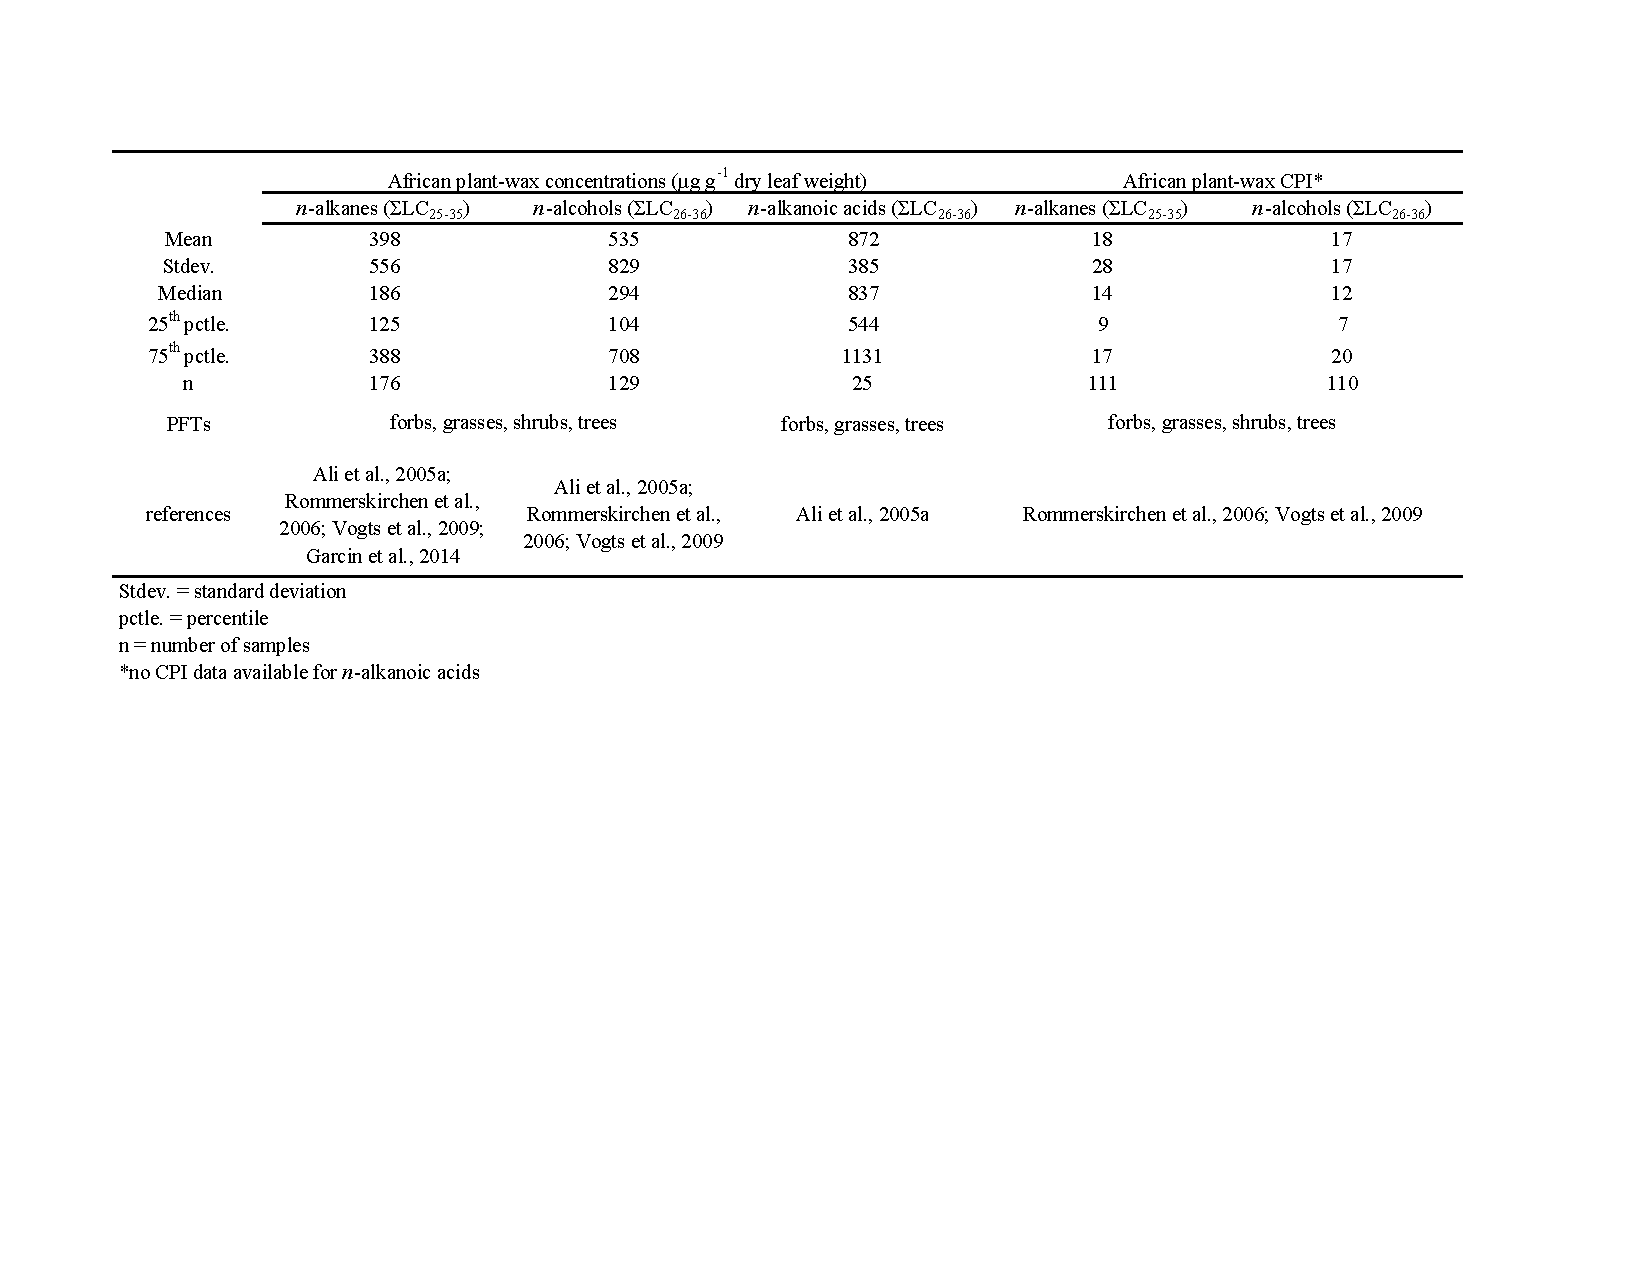
\includegraphics{Thesis_Tables/Ch4Tab4}
	\label{Ch4Tab:4} 
\end{sidewaystable}

% Figure 9
\begin{figure}[p]
	\makebox[\textwidth][c]{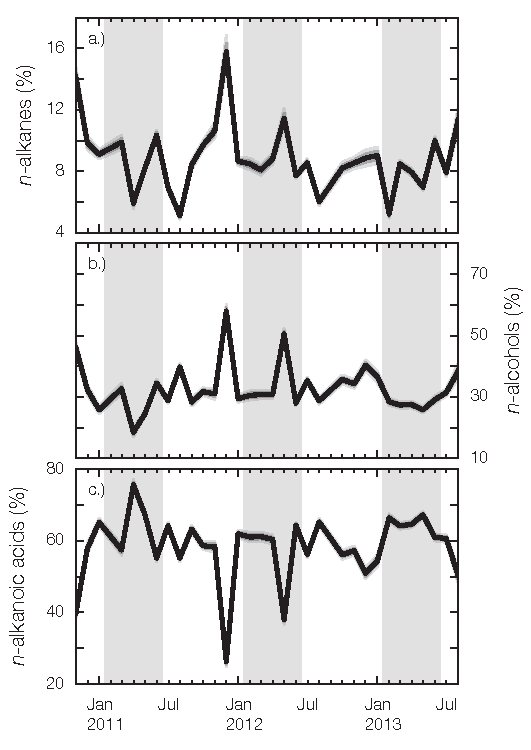
\includegraphics[]{Thesis_Figures/Ch4Fig9}}
	\caption[Time-series plots of compound-class contribution]{Time series plots of the fractional contribution to the plant-wax \textit{n}-alkyl lipid total by \textit{(A)} $\Sigma$LC\textsubscript{25-35} \textit{n}-alkanes, \textit{(B)} $\Sigma$LC\textsubscript{26-36} \textit{n}-alcohols, and \textit{(C)} $\Sigma$LC\textsubscript{26-36} \textit{n}-alkanoic acids. Dark gray shading represents $\pm 1 \sigma$ regression uncertainty, and light gray shading represents 95\% CI. Periods when f\textsubscript{south} > 39\% are indicated by gray boxes.}
	\label{Ch4Fig:9} 
\end{figure}

\textit{n}-Alkane concentrations, ACL, CPI, and \ce{\delta^{13}C} values show little to no correlation with discharge (Figure \ref{Ch4Fig:4}, \ref{Ch4Fig:5}A--C), indicating that exported \textit{n}-alkane signals do not respond to environmental changes on seasonal timescales. In contrast, if \textit{n}-alkanes were dominated by a recently entrained local signal, discharge should exhibit a strong control on molecular concentration/distribution and/or isotopic composition due to temporal variability in northern vs. southern hemisphere tributary contributions and their corresponding PFT signatures (Figure \ref{Ch4Fig:1}, \ref{Ch4Fig:2}B). However, this is not observed. This lack of correlation between \textit{n}-alkane concentration, ACL, and discharge likely explains the similarly low and invariant P\textsubscript{aq} values (Table \ref{Ch4Tab:S2}), as \textit{Cuvette Congolaise} macrophytes do not contribute significantly to exported \textit{n}-alkanes during periods of high northern hemisphere discharge.

Differences in isotope composition between homologues contain additional information related to residence time and end-member contribution in river systems with stable ecosystems and discharge source regions. Integration over multiple source regions with unique \textit{n}-alkane homologue distributions should result in large \ce{\delta^{13}C} variability with chain length. For example, \citet{Agrawal:2014fl} observed a consistent increase in \ce{\delta^{13}C} values with chain length of up to $\approx 6$\textperthousand\ between C\textsubscript{24} and C\textsubscript{32} \textit{n}-alkanoic acids in a sediment core taken from the Ganges floodplain at the base of the Himalayas. Additionally, they describe a unique "bimodal" concentration distribution with a maximum at C\textsubscript{24} and with significantly lower C\textsubscript{26}/C\textsubscript{28} and higher C\textsubscript{30}/C\textsubscript{32} concentrations than would be expected based on the distributions in modern Ganges suspended sediments \citep{Galy:2011ix}. Taken together, \citet{Agrawal:2014fl} use these results as evidence for degradation of Himalayan C\textsubscript{3} \textit{n}-alkanoic acids and replacement by local floodplain C\textsubscript{4}-derived compounds, and conclude that C\textsubscript{26}/C\textsubscript{28} better retain a headwater signal while C\textsubscript{30}/C\textsubscript{32} exhibit significant overprinting due to higher production of the longer-chain homologues by local C\textsubscript{4} grasses.

In the Congo River, integration of \textit{n}-alkanes over multiple source regions should result in a similarly large \ce{\delta^{13}C} difference across homologues and lower correlation between homologue concentrations, as is observed (Table \ref{Ch4Tab:1}; Figure \ref{Ch4Fig:3}D, \ref{Ch4Fig:4}D). Depleted \ce{\delta^{13}C} values for C\textsubscript{29} and C\textsubscript{31} \textit{n}-alkane confirm the importance of a C\textsubscript{3} source to these compounds, while relatively \ce{^{13}C}-enriched C\textsubscript{33} and, especially, C\textsubscript{35} values indicate a larger contribution by C\textsubscript{4} grasses with increasing chain length. This agrees with measurements of individual plant leaves, as African gramminoids have been shown to produce higher relative concentrations of C\textsubscript{33} (C\textsubscript{35} not measured) as compared to African trees and forbs \citep{Rommerskirchen:2006gr,Vogts:2009fb}. Using a typical end-member \textit{n}-alkane isotopic value of $-35$\textperthousand\ for C\textsubscript{3} and $-22$\textperthousand\ for C\textsubscript{4} plants \citep[\textit{e.g.}][]{Castaneda:2011jb}, this results in a C\textsubscript{4} contribution as high as $69 \pm 6$\% to C\textsubscript{35} \textit{n}-alkane and as low as $8 \pm 4$\% to C\textsubscript{29} \textit{n}-alkane, while remote-sensing results indicate that catchment-wide C\textsubscript{4} gramminoid coverage is $\approx 14$\% \citep[Figure \ref{Ch4Fig:1}B;][]{Still:2010wh}. However, we note that remote sensing likely underestimates C\textsubscript{4} coverage in forested areas, as C\textsubscript{4} plants are masked by C\textsubscript{3} forest canopy.

% Figure 10
\begin{figure}[p]
	\makebox[\textwidth][c]{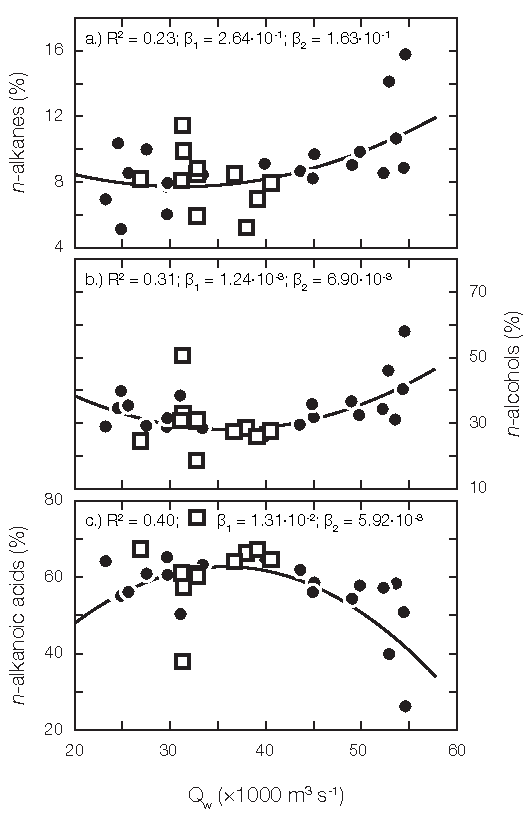
\includegraphics[]{Thesis_Figures/Ch4Fig10}}
	\caption[Correlation between compound-class contribution and discharge]{Fractional contribution by \textit{(A)} $\Sigma$LC\textsubscript{25-35} \textit{n}-alkanes, \textit{(B)} $\Sigma$LC\textsubscript{26-36} \textit{n}-alcohols, and \textit{(C)} $\Sigma$LC\textsubscript{26-36} \textit{n}-alkanoic acids plotted vs. Congo River discharge (Q\textsubscript{w}) measured at Brazzaville/Kinshasa. Black line is the quadratic WLS regression line. $R^2$ values and significance $p$-values for linear ($\beta_1$) and quadratic ($\beta_2$) parameters are reported for each regression. Samples collected when f\textsubscript{south} > 39\% are plotted as white squares, and samples collected when f\textsubscript{south} $\leq$ 39\% are plotted as black circles. Uncertainty ($\pm 1 \sigma$) is smaller than the symbols for all data points.}
	\label{Ch4Fig:10} 
\end{figure}

Spatially, C\textsubscript{4}-bearing savannah and woodland/shrubland ecosystems are mostly located at the northern and southern extremes of the catchment, above $5$\textdegree N and between $5-10$\textdegree S, while C\textsubscript{3}-dominated evergreen forest, deciduous/montane forest, and swamp forest occupy the central region (Figure \ref{Ch4Fig:1}). This geographic separation indicates a variable apparent integration region for \textit{n}-alkane homologues, with the longest chain-length \textit{n}-alkanes biasing toward headwater regions due to higher production by gramminoids. Additionally, observed negative correlations between C\textsubscript{27}--C\textsubscript{33} \textit{n}-alkane concentrations and \ce{\delta^{13}C} values (Table \ref{Ch4Tab:3}) are further evidence for an overprinting of distal C\textsubscript{4} sources during transit. This relationship is strongest for C\textsubscript{29} and C\textsubscript{31} ($r = -0.74$, $-0.65$), consistent with significant production of these compounds in C\textsubscript{3} trees and forbs \citep{Rommerskirchen:2006gr,Vogts:2009fb}. In contrast, C\textsubscript{35} \ce{\delta^{13}C} values are uncorrelated with concentration, further indicating a predominantly headwater C\textsubscript{4} source to this compound, irrespective of concentration. While regions of mosaic savannah/grassland and deciduous woodland/shrubland exist near the sampling site, especially in left-bank tributaries (Figure \ref{Ch4Fig:1}), this contribution is likely minimal. If local C\textsubscript{4} sources were important, this would lead to \ce{^{13}C}-enrichment of all \textit{n}-alkane homologues, especially during periods of predominantly southern hemisphere discharge, which is not observed (Figure \ref{Ch4Fig:4}D).

Biasing of C\textsubscript{33} and C\textsubscript{35} \textit{n}-alkanes toward a headwater C\textsubscript{4} signal agrees with time series measurements of the Oubangui River at Bangui Station ($4.36$\textdegree N, $18.55$\textdegree E; Figure \ref{Ch4Fig:1}). \citet{Bouillon:2012cw} show enriched POC \ce{\delta^{13}C} values ($-26.2 \pm 0.4$\textperthousand, $n = 11$) during periods of high discharge, when autochthonous production is negligible, as this headwater tributary contains significant amounts of dry woody savannah ecosystem coverage. Additionally, enriched POC \ce{\delta^{13}C} values up to $-22.8$\textperthousand\ have been reported for a small savannah tributary to the Oubangui River, while the nearby savannah-dominated Niari River exhibits POC \ce{\delta^{13}C} values as high as $-18.6$\textperthousand\ \citep{Mariotti:1991vx,Bouillon:2014ko}. In contrast, the Congo main-stem near Brazzaville displays more depleted POC \ce{\delta^{13}C} values, averaging $-28.2 \pm 0.4$\textperthousand\ \citep[$n = 5$;][]{Spencer:2012en}.

Additional evidence for variable spatial integration of \textit{n}-alkane homologues comes from a positive correlation between the \ce{\delta^{13}C} values of \textit{n}-alkanoic acids/\textit{n}-alcohols and their corresponding \textit{n}-alkanes (\textit{i.e.} $n - 1$), as decarboxylation and dehydration of functionalized \textit{n}-alkyl lipids has been shown to occur rapidly in sediments \citep{Cranwell:1981vg,Sun:1994wj,Sun:1997wr,Hoefs:2002wu}. Such relationships are especially strong between C\textsubscript{30}/C\textsubscript{32} \textit{n}-alcohol and \textit{n}-alkanoic acid and C\textsubscript{29}/C\textsubscript{31} \textit{n}-alkane ($r$ up to $0.75$; Table \ref{Ch4Tab:2}), indicating that diagenetic contribution by functionalized C\textsubscript{3} plant waxes contributes to the overprinting of these compounds during transit. Taken together, the observed depleted \ce{\delta^{13}C} values, negative correlations between \ce{\delta^{13}C} and concentration, and positive \ce{\delta^{13}C} correlations with corresponding functionalized lipids indicate that C\textsubscript{29} and C\textsubscript{31} \textit{n}-alkane exhibit significant overprinting during fluvial transit and bias toward a more local signal. In contrast, enriched \ce{\delta^{13}C} values and weaker correlation between \ce{\delta^{13}C} and concentration for C\textsubscript{33} and, especially, C\textsubscript{35} \textit{n}-alkanes are strong evidence that these homologues better retain a headwater signal.

\subsection{\textit{n}-Alcohols and \textit{n}-alkanoic acids are controlled by recently entrained local sources}\label{Ch4Sec:52}

Contrary to \textit{n}-alkanes, carbon-normalized concentrations of plant-wax \textit{n}-alcohols and \textit{n}-alkanoic acids in Congo River POC are equal to or greater than the highest observed values in any large river system to date \citep{Saliot:2001un,vanDongen:2008kj,Galy:2011ix,Tao:2015bq}. Such high \textit{n}-alcohol:\textit{n}-alkane ($3.8 \pm 0.9$) and \textit{n}-alkanoic acid:\textit{n}-alkane ($7.1 \pm 2.5$) ratios in suspended sediments contrast with the overlapping range in concentrations between compound classes found in African plants (Table \ref{Ch4Tab:4}). Additionally, despite an identical range in CPI for \textit{n}-alkanes and \textit{n}-alcohols (no \textit{n}-alkanoic data exist) in individual African plant leaves (Table  \ref{Ch4Tab:4}), both functionalized compound classes exhibit higher CPI values than do \textit{n}-alkanes in suspended sediment (Tables \ref{Ch4Tab:S2}--\ref{Ch4Tab:S4}), as diagenetic degradation has been shown to lower CPI \citep{Meyers:1993vwa}.

Assuming no pervasive biases against the transfer of \textit{n}-alkanes into soils and subsequent entrainment into streams, high concentrations and CPI values of functionalized lipids relative to \textit{n}-alkanes, despite similar input composition from plants (Table \ref{Ch4Tab:4}), supports the hypothesis that exported \textit{n}-alcohols and \textit{n}-alkanoic acids are mostly sourced from local surface soils with less exposure to diagenesis prior to export. Functionalized wax lipids are known to experience rapid diagenetic dehydration and decarboxylation in sediments \citep{Meyers:1993up,Sun:1994wj,Canuel:1996ta,Sun:1997wr}. For example, \citet{Sun:1997wr} report that 90\% of $^{14}$C-labeled C\textsubscript{16} \textit{n}-alkanoic acids (labeled in the methyl position) are degraded due to decarboxylation within 80 days during incubation experiments. While C\textsubscript{16} \textit{n}-alkanoic acid is produced ubiquitously in the environment, rapid degradation has additionally been observed for plant-wax-specific \textit{n}-alkanoic acids (\textit{i.e.} C\textsubscript{26}--C\textsubscript{30}) and \textit{n}-alcohols (C\textsubscript{26}--C\textsubscript{30}) upon re-exposure of sediments to oxygen \citep{Hoefs:2002wu}. \textit{n}-Alkanoic acids and \textit{n}-alcohols frequently exhibit the lowest preservation of all lipids in marine and lacustrine sediments and have been observed to degrade at faster rates than bulk OC \citep{Cranwell:1981vg,Meyers:1993vwa}. However, lipid preservation is additionally a function of sediment mineralogy, as sorptive interactions with mineral surfaces have been shown to stabilize labile OC \citep[\textit{e.g.}][]{Keil:1994hb,Mayer:1994wn}.

Isotopic evidence further indicates a predominantly local source, as these compound classes exhibit depleted \ce{\delta^{13}C} values for all plant-wax homologues (average $\leq -31.3$\textperthousand\ and $-30.8$\textperthousand, respectively; Figure \ref{Ch4Fig:3}E--F). Using a C\textsubscript{3} end-member value of -35\textperthousand\ and a C\textsubscript{4} end-member value of -22\textperthousand, as above \citep{Castaneda:2011jb}, this leads to a minimum C\textsubscript{3} contribution to \textit{n}-alcohols of $73 \pm 5$\% (C\textsubscript{32}) and $68 \pm 6$\% to \textit{n}-alkanoic acids (C\textsubscript{26}). However, this is likely an underestimate, as relatively enriched \ce{\delta^{13}C} values for individual C\textsubscript{3} angiosperm lipids have been reported \citep[\textit{i.e.} up to $-30$\textperthousand; ][]{Diefendorf:2011hg,Garcin:2014hg}. Isotopic evidence therefore indicates that functionalized lipids are predominantly sourced from local C\textsubscript{3} ecosystems, as C\textsubscript{4} land cover is mostly limited to distal headwater regions (Figure \ref{Ch4Fig:1}B). Similar to \textit{n}-alkanes, regions of mosaic savannah/grassland and deciduous woodland/shrubland near the sampling site likely do not contribute significantly to exported \textit{n}-alcohols and \textit{n}-alkanoic acids, as this would lead to a \ce{^{13}C}-enrichment during southern hemisphere dominated discharge periods, which is not observed (Figure \ref{Ch4Fig:6}D, \ref{Ch4Fig:7}D, \ref{Ch4Fig:8}).

Unlike longer chain homologues, autochthonous production of C\textsubscript{24} \textit{n}-alcohol has been observed in freshwater phytoplankton \citep{Volkman:1998tk,Volkman:1999tq,Xu:2007jk}, and is likely a significant source of this compound in our sample set. This is supported by depleted \ce{\delta^{13}C} values (Figure \ref{Ch4Fig:3}E) and a strong positive relationship with discharge (Figure \ref{Ch4Fig:8}A). 

If dissolved inorganic carbon (DIC) is \ce{^{13}C}-depleted relative to atmospheric \ce{CO2}, autochthonous contribution will lead to lower observed \ce{\delta^{13}C} values for C\textsubscript{24} \textit{n}-alcohol, especially during periods of low discharge when phytoplankton production is highest. While no DIC \ce{\delta^{13}C} values exist at our sampling site, low- and rising-water values at Bangui station average $-10.0 \pm 2.2$\textperthousand\ \citep[$n = 30$;][]{Bouillon:2012cw,Bouillon:2014ko}.  Additionally, C\textsubscript{24} \textit{n}-alcohol \ce{\delta^{13}C} values are strongly correlated with those of C\textsubscript{22} \textit{n}-alcohol ($R^2 = 0.75$, $p$-value = $4.0 \times 10^{-10}$; not shown), the dominant lipid in freshwater phytoplankton \citep{Volkman:1998tk,Volkman:1999tq,Xu:2007jk}, and are uncorrelated with longer chain-length values ($p$-value > $0.05$; not shown). While a slight \ce{\delta^{13}C} vs. discharge correlation is observed for other compounds (\textit{i.e.} C\textsubscript{26} \textit{n}-alcohol, C\textsubscript{24} and C\textsubscript{28} \textit{n}-alkanoic acid; Figure \ref{Ch4Fig:8}), these homologues are consistently $\approx 3-5$\textperthousand\ enriched relative to C\textsubscript{24} \textit{n}-alcohol, indicating minimal autochthonous contribution.

Further evidence for a local, C\textsubscript{3} signal to functionalized \textit{n}-alkyl lipids comes from the fact that \ce{\delta^{13}C} values show significantly weaker negative correlation with lipid concentrations than do \textit{n}-alkanes, with the exception of C\textsubscript{24} \textit{n}-alcohol and C\textsubscript{24} \textit{n}-alkanoic acid (Table \ref{Ch4Tab:3}). As with \textit{n}-alkanes, a negative correlation would indicate addition of C\textsubscript{3} material to a background C\textsubscript{4} signal during transit. However, this is not the case, especially for longer chain-length homologues (\textit{i.e.} C\textsubscript{28+}), indicating negligible contribution by C\textsubscript{4}-dominated headwater ecosystems to measured compounds and therefore a smaller apparent integration region than is observed for \textit{n}-alkanes, especially C\textsubscript{33} and C\textsubscript{35}. African C\textsubscript{4} gramminoids exhibit similar \textit{n}-alcohol and \textit{n}-alkanoic acid production rates as African forbs, shrubs, and trees \citep{Ali:2005ab,Rommerskirchen:2006gr,Vogts:2009fb}, indicating that this signal is not due to a source effect. Rather, it is likely the result of quantitative diagenetic degradation of headwater functionalized \textit{n}-alkyl lipids during fluvial transit \citep{Cranwell:1981vg,Meyers:1993vwa,Sun:1997wr,Hoefs:2002wu,vanDongen:2008kj}. In addition, a low spread in \ce{\delta^{13}C} values across plant-wax chain-lengths (Figure \ref{Ch4Fig:3}E--F) and strong positive correlations between homologue concentrations (Table \ref{Ch4Tab:1}) precludes significant spatial integration of multiple PFTs with unique molecular distribution and isotope composition \citep[\textit{c.f.}][]{Agrawal:2014fl}.

Additionally, we observe large seasonal variability in \textit{n}-alcohol and \textit{n}-alkanoic acid relative contribution (Figure \ref{Ch4Fig:9}), indicating a change in functionalized lipid source in response to seasonal hydrology. This is consistent with the above evidence that these compounds are sourced from recently entrained OC and integrate a mostly local signal. \textit{n}-Alcohol relative contribution displays a statistically significant increase during \textit{Cuvette Congolaise} dominated periods, balanced by an equal decrease in \textit{n}-alkanoic acids (Figure \ref{Ch4Fig:10}). These results agree with literature measurements of individual plants, as macrophytes display considerably higher \textit{n}-alcohol production rates than do other PFTs \citep{Ficken:1998vs,Ficken:2000wq,Bugalho:2004kj,Ali:2005ab,Ali:2005cr,Aichner:2010bk,Gao:2011dj,Diefendorf:2011hg,Wang:2012fb,Gao:2014bk}.

It has been shown that the Congo main-stem and a range of tributaries bias toward swamp-forest-like chemical properties during periods of high discharge, indicating an increased contribution by this ecosystem to exported organic carbon \citep{Wang:2013js,Mann:2014jx}. These observations, combined with an increase in \textit{n}-alcohol fractional contribution, are strong evidence for a significant increase in \textit{Cuvette Congolaise} contribution to functionalized \textit{n}-alkyl lipids during periods of high northern hemisphere discharge. Thus, our results indicate that this geographically small region \citep[4\% coverage;][]{Mayaux:2004uw} exhibits a dominant control on the composition of exported functionalized \textit{n}-alkyl lipids in response to seasonal changes in hydrology. However, a lack of significant \ce{\delta^{13}C} variability across the time series for any functionalized plant-wax lipid (Figure \ref{Ch4Fig:6}D, \ref{Ch4Fig:7}D) indicates that their \ce{\delta^{13}C} values are not a sensitive tracer for changes in \textit{n}-alkyl lipid source on these timescales.

\subsection{Comparison to other river basins and global significance}

Variable spatiotemporal integration of \textit{n}-alkane homologues and a local, recently entrained \textit{n}-alcohol/\textit{n}-alkanoic acid signal is a feature not limited to the Congo River catchment. For example, isotopic and molecular signals of \textit{n}-alkanes and \textit{n}-alkanoic acids show differential contribution by C\textsubscript{4} grasses during transport in the Ganges River through the floodplain \citep{Galy:2011ix}. Using the data of \citet{Galy:2011ix}, we compare the concentration-weighted Himalayan plant-wax signal to that just before the confluence with the Brahmaputra River in Bangladesh, noting that sediment fluxes are nearly identical in all major Himalayan tributaries \citep{Andermann:2012br}.

Himalayan plant-wax \textit{n}-alkanes (C\textsubscript{25}--C\textsubscript{35}) and \textit{n}-alkanoic acids (C\textsubscript{26}--C\textsubscript{34}) display nearly identical \ce{\delta^{13}C} composition, averaging $-32.1$\textperthousand\ and $-32.3$\textperthousand\ respectively, with similar spread between chain-lengths of $1.8$\textperthousand\ and $1.4$\textperthousand. In contrast, downstream Ganges \textit{n}-alkanoic acid \ce{\delta^{13}C} values are enriched by an average of $1.3$\textperthousand\ relative to \textit{n}-alkanes. Additionally, isotopic spread between chain lengths remains constant for \textit{n}-alkanoic acids (\textit{i.e.} $1.4$\textperthousand), but increases to $3.5$\textperthousand\ for \textit{n}-alkanes, while ACL of both compound classes increases by $\approx 1$ unit. Combined, these results indicate that C\textsubscript{3} \textit{n}-alkanoic acids sourced in the Himalayan range are quantitatively replaced by a mixed C\textsubscript{3}/C\textsubscript{4} floodplain signal independent of chain length. In contrast, \textit{n}-alkanes display differential contribution by a floodplain signal across chain lengths, with C\textsubscript{33}/C\textsubscript{35} showing the most influence. Quantitative \textit{n}-alkanoic acid replacement during floodplain transit agrees with the results of \citet{Agrawal:2014fl}, which already show significant overprinting near the base of the Himalayan range. Thus, despite large differences in sediment erosion rates and biospheric carbon yields between the Congo and Ganges rivers \citep{Galy:2015fx}, exported plant waxes display similar behavior in these two catchments.

In addition to the Ganges River, a large spread in \textit{n}-alkane \ce{\delta^{13}C} values with chain-length has been observed in settings such as Cameroonian lacustrine and Washington margin surface sediments \citep{Feng:2013iv,Garcin:2014hg} and a Zambezi River sedimentary archive \citep{Wang:2013jz}. Differential contribution by C\textsubscript{3}/C\textsubscript{4} plants to \textit{n}-alkanes with chain length therefore appears to be a common phenomenon. We suggest that \ce{\delta^{13}C} measurement of multiple \textit{n}-alkane chain lengths can be used to address nonlinear PFT mixing during transport \citep{Garcin:2014hg}, as C\textsubscript{33} and, especially, C\textsubscript{35} bias almost exclusively toward a C\textsubscript{4} end-member, opposite to C\textsubscript{29} and C\textsubscript{31}.

Additionally, differential sourcing between compound classes (\textit{i.e.} functionalized vs. \textit{n}-alkanes) appears to be common in river catchments spanning multiple ecosystems. Thus, in addition to \textit{n}-alkanes, measurement of \textit{n}-alcohols and \textit{n}-alkanoic acids in river sediments and fluvially dominated sedimentary archives can be utilized to address geospatial PFT distribution within the catchment, as functionalized lipids will bias toward a local signal \citep[\textit{e.g.}][this study]{Galy:2011ix,Ponton:2014jr}.

\section{Conclusion}

We report concentrations and \ce{\delta^{13}C} values of three classes of dominantly plant-derived \textit{n}-alkyl lipids from a 34-month time series of Congo River suspended sediments. Our results show that \textit{n}-alkanoic acid and \textit{n}-alcohol concentrations are equal to or greater than the highest OC-normalized concentrations in large fluvial systems reported to date. In contrast, \textit{n}-alkanes concentrations are lower than those reported in other major rivers. Spread in \textit{n}-alcohol and \textit{n}-alkanoic acid \ce{\delta^{13}C} values between long-chain homologues is lower than observed in other major rivers, while \textit{n}-alkanes exhibit up to $\approx 8$\textperthousand\ enrichment with increasing chain length.

These data indicate that \textit{n}-alkanoic acids and \textit{n}-alcohols are sourced from local, C\textsubscript{3}-dominated ecosystems, consistent with the idea that high reactivity of functional groups precludes significant spatial integration of these compounds. In contrast, \textit{n}-alkane homologues variably integrate over a wide range of ecosystems with increasing contribution by distal C\textsubscript{4}-dominated savannah and woodland/shrubland source regions to the longest chain-length compounds. Strong seasonal shifts in relative \textit{n}-alkanoic acid and \textit{n}-alcohol concentrations indicate that functionalized lipids respond rapidly to changes in hydrological regime. This signal, however, is not reflected in \ce{\delta^{13}C} values. During periods of highest northern hemisphere discharge, an increase in fractional \textit{n}-alcohol contribution and decrease in \textit{n}-alkanoic acid contribution suggest a strong bias towards a local swamp-forest signal. \textit{n}-Alkanes are less affected by seasonal changes in discharge, further indicating that these compounds integrate over a larger source region.

Consequently, we suggest that simultaneous measurement of multiple \textit{n}-alkyl lipid classes and chain lengths in down-core samples will likely provide better geospatial resolution for paleo-ecosystem reconstruction due to their differential integration regions and C\textsubscript{3}/C\textsubscript{4} biases.

%\section*{Acknowledgements}

%We thank Carl Johnson (WHOI), Sarah Rosengard (WHOI), and Ralph Kreutz (MARUM) for laboratory assistance. V.V.G. was partly supported by the US National Science Foundation, grants OCE-0851015 and OCE-0928582; J.D.H. was supported by the National Science Foundation Graduate Research Fellowship under Grant No. 2012126152; E.S was supported by the DFG Research Center/Cluster of Excellence "The Ocean in the Earth System" at MARUM -- Center for Marine Environmental Science, University of Bremen. This manuscript benefited greatly through the constructive comments of Aaron Diefendorf, Clayton Magill, one anonymous reviewer, and associate editor Thomas Bianchi.

\clearpage

\section{Supplementary Material}

\subsection{Supplementary Tables}

% Reset table counter
\renewcommand\thetable{\thechapter.S\arabic{table}}    
\setcounter{table}{0}

% Change caption justification
\captionsetup[table]{justification=raggedright,singlelinecheck=off}

All supplementary tables for this chapter are available in the open-source \emph{Pangaea} database at the following link: \url{https://doi.pangaea.de/10.1594/PANGAEA.864152}

% Table S1
\begin{table}[h!]
	\caption[Congo River environmental parameters]{Environmental parameters for the Congo River recorded near Brazzaville/Kinshasa during the sampling period (November 2010 -- August 2013).}
	\label{Ch4Tab:S1} 
\end{table}

% Table S2
\begin{table}[h!]
	\caption[\textit{n}-alkane concentrations, ACL, CPI, and P\textsubscript{aq}]{Concentrations of \textit{n}-alkanes, average chain length, and carbon preference index during the sampling period (November 2010 -- August 2013).}
	\label{Ch4Tab:S2} 
\end{table}

% Table S3
\begin{table}[h!]
	\caption[\textit{n}-alcohol concentrations, ACL, and CPI]{Concentrations of \textit{n}-alcohols, average chain length, and carbon preference index during the sampling period (November 2010 -- August 2013).}
	\label{Ch4Tab:S3} 
\end{table}

% Table S4
\begin{table}[h!]
	\caption[\textit{n}-alkanoic acid concentrations, ACL, and CPI]{Concentrations of \textit{n}-alkanoic acids, average chain length, and carbon preference index during the sampling period (November 2010 -- August 2013).}
	\label{Ch4Tab:S4} 
\end{table}

% Table S5
\begin{table}[h!]
	\caption[\textit{n}-alkane \ce{\delta^{13}C} values]{\ce{\delta^{13}C} values of \textit{n}-alkanes during the sampling period (November 2010 -- August 2013).}
	\label{Ch4Tab:S5} 
\end{table}

% Table S6
\begin{table}[h!]
	\caption[\textit{n}-alcohol \ce{\delta^{13}C} values]{\ce{\delta^{13}C} values of \textit{n}-alcohols during the sampling period (November 2010 -- August 2013).}
	\label{Ch4Tab:S6} 
\end{table}

% Table S7
\begin{table}[h!]
	\caption[\textit{n}-alkanoic acid \ce{\delta^{13}C} values]{\ce{\delta^{13}C} values of \textit{n}-alkanoic acids during the sampling period (November 2010 -- August 2013).}
	\label{Ch4Tab:S7} 
\end{table}

% Table S8
\begin{table}[h!]
	\caption[Compound class relative contributions]{Relative compound class contributions to total \textit{n}-alkyl lipids during the sampling period (November 2010 -- August 2013).}
	\label{Ch4Tab:S8} 
\end{table}

% Reset for future chapters
\renewcommand\thetable{\thechapter.\arabic{table}}

% Reset caption justification
\captionsetup[table]{justification=justified}
   
